\documentclass[11pt,fleqn]{book} % Default font size and left-justified equations

\newcommand \subjectName {Computer Networks and Internet}
\newcommand \subjectNumber {104353}
\newcommand \subjectDegree {Data Engineering}
\newcommand \subjectYear {1$^\textrm{st}$}
\newcommand \guideVersion {2025}

\usepackage[top=1.5cm,bottom=1cm,left=2cm,right=2cm,headsep=10pt,a4paper]{geometry} % Page margins

\usepackage[dvipsnames]{xcolor}
\definecolor{color1}{RGB}{243,102,25} % Define the orange color used for highlighting throughout the book
\definecolor{color2}{RGB}{0,100,140} % Define the orange color used for highlighting throughout the book
\definecolor{color3}{RGB}{40,100,35} % Define the orange color used for highlighting throughout the book
\definecolor{color4}{RGB}{243,102,25} % Define the orange color used for highlighting throughout the book

\usepackage{imakeidx} % Required to make an index (needed BEFORE hyperref)
\indexsetup{level=\section*,noclearpage}
\makeindex[columns=3,title={}] % Tells LaTeX to create the files required for indexing
\usepackage{hyperref}
\hypersetup{hidelinks,colorlinks=true,linktoc=all,breaklinks=true,allcolors=color2,bookmarksopen=false,pdftitle={Study Guide: \subjectName},pdfauthor={Miguel Hernández-Cabronero <miguel.hernandez@uab.cat>}}
\usepackage{pdfcomment}


\usepackage{graphicx} % Required for including pictures
\graphicspath{{style/}{chapters/fig/}} % Specifies the directory where pictures are stored

\usepackage[utf8]{inputenc} % Required for including letters with accents
\usepackage[LGR,T1]{fontenc}
\newcommand{\textgreek}[1]{\begingroup\fontencoding{LGR}\selectfont#1\endgroup}
\usepackage{todonotes}
\usepackage{schedule}
\usepackage{multicol}
\usepackage{pgf-pie}
\usepackage[skip=6pt plus1pt, indent=0pt]{parskip}
\usepackage{comment}
\usepackage{xifthen}
\usepackage{wrapfig}
\usepackage{circledtext}
\usepackage{textcomp}
\usepackage{moresize}
\usepackage{lipsum} % Inserts dummy text
\usepackage{tikz} % Required for drawing custom shapes
\usepackage[english]{babel} % English language/hyphenation
\usepackage{enumitem} % Customize lists
\setlist{nolistsep} % Reduce spacing between bullet points and numbered lists
\usepackage{booktabs} % Required for nicer horizontal rules in tables
\usepackage{listings}
\usepackage{minted}
\usepackage{circledsteps}
\usepackage{bytefield}
\usepackage{qrcode}


%----------------------------------------------------------------------------------------
%	FONTS
%----------------------------------------------------------------------------------------

\usepackage{avant} % Use the Avantgarde font for headings
%\usepackage{times} % Use the Times font for headings
% \usepackage{mathptmx} % Use the Adobe Times Roman as the default text font together with math symbols from the Sym­bol, Chancery and Com­puter Modern fonts
\renewcommand{\familydefault}{\sfdefault}

\usepackage{microtype} % Slightly tweak font spacing for aesthetics
\usepackage[T1]{fontenc} % Use 8-bit encoding that has 256 glyphs

%----------------------------------------------------------------------------------------
%	BIBLIOGRAPHY AND INDEX
%----------------------------------------------------------------------------------------

% \usepackage{csquotes}
% \usepackage[style=alphabetic,citestyle=numeric,sorting=nyt,sortcites=true,autopunct=true,autolang=hyphen,hyperref=true,abbreviate=false,backref=true,backend=biber,defernumbers=true]{biblatex}
% \left\addbibresource{bibliography.bib} % BibTeX bibliography file
% \defbibheading{bibempty}{}

\usepackage{calc} % For simpler calculation - used for spacing the index letter headings correctly

%----------------------------------------------------------------------------------------
%	MAIN TABLE OF CONTENTS
%----------------------------------------------------------------------------------------

\usepackage{titletoc} % Required for manipulating the table of contents

\contentsmargin{0cm} % Removes the default margin

% Part text styling
\titlecontents{part}[0cm]
{\addvspace{20pt}\centering\large\bfseries}
{}
{}
{}

% Chapter text styling
\titlecontents{chapter}[1.25cm] % Indentation
{\addvspace{12pt}\large\sffamily\bfseries} % Spacing and font options for chapters
{\color{color1!60}\contentslabel[\Large\thecontentslabel]{1.25cm}\color{color1}} % Chapter number
{\color{color1}}  
{\color{color1!60}\normalsize\;\titlerule*[.5pc]{.}\;\thecontentspage} % Page number

% Section text styling
\titlecontents{section}[1.25cm] % Indentation
{\addvspace{3pt}\sffamily\bfseries} % Spacing and font options for sections
{\contentslabel[\thecontentslabel]{1.25cm}} % Section number
{}
{\hfill\color{black}\thecontentspage} % Page number
[]

% Subsection text styling
\titlecontents{subsection}[1.25cm] % Indentation
{\addvspace{1pt}\sffamily\small} % Spacing and font options for subsections
{\contentslabel[\thecontentslabel]{1.25cm}} % Subsection number
{}
{\ \titlerule*[.5pc]{.}\;\thecontentspage} % Page number
[]

% List of figures
\titlecontents{figure}[0em]
{\addvspace{-5pt}\sffamily}
{\thecontentslabel\hspace*{1em}}
{}
{\ \titlerule*[.5pc]{.}\;\thecontentspage}
[]

% List of tables
\titlecontents{table}[0em]
{\addvspace{-5pt}\sffamily}
{\thecontentslabel\hspace*{1em}}
{}
{\ \titlerule*[.5pc]{.}\;\thecontentspage}
[]

%----------------------------------------------------------------------------------------
%	MINI TABLE OF CONTENTS IN PART HEADS
%----------------------------------------------------------------------------------------

% Chapter text styling
\titlecontents{lchapter}[0em] % Indenting
{\addvspace{15pt}\large\sffamily\bfseries} % Spacing and font options for chapters
{\color{color1}\contentslabel[\Large\thecontentslabel]{1.25cm}\color{color1}} % Chapter number
{}  
{\color{color1}\normalsize\sffamily\bfseries\;\titlerule*[.5pc]{.}\;\thecontentspage} % Page number

% Section text styling
\titlecontents{lsection}[0em] % Indenting
{\sffamily\small} % Spacing and font options for sections
{\contentslabel[\thecontentslabel]{1.25cm}} % Section number
{}
{}

% Subsection text styling
\titlecontents{lsubsection}[.5em] % Indentation
{\normalfont\footnotesize\sffamily} % Font settings
{}
{}
{}

%----------------------------------------------------------------------------------------
%	PAGE HEADERS
%----------------------------------------------------------------------------------------

\usepackage{fancyhdr} % Required for header and footer configuration
\usepackage{lastpage}

\pagestyle{fancy}
\renewcommand{\chaptermark}[1]{\markboth{\sffamily\normalsize\bfseries\chaptername\ \thechapter.\ #1}{}} % Chapter text font settings
\renewcommand{\sectionmark}[1]{\markright{\sffamily\normalsize\thesection\hspace{5pt}#1}{}} % Section text font settings
\fancyhf{} \fancyhead[LE,RO]{\sffamily\normalsize} % Font setting for the page number in the header
\fancyfoot[C]{\raisebox{0.25cm}{\thepage\ {\color{color1}/}\ \pageref*{LastPage}}}
\fancyhead[L]{Study Guide{\color{color1}:} \subjectName}
\fancyhead[R]{\thepage\ {\color{color1}/}\ \pageref*{LastPage}}

\renewcommand{\headrulewidth}{0.5pt} % Width of the rule under the header
\addtolength{\headheight}{2.5pt} % Increase the spacing around the header slightly
\renewcommand{\footrulewidth}{0pt} % Removes the rule in the footer
\fancypagestyle{plain}{\fancyhead{}\renewcommand{\headrulewidth}{0pt}} % Style for when a plain pagestyle is specified

% Removes the header from odd empty pages at the end of chapters
\makeatletter
\renewcommand{\cleardoublepage}{
% \clearpage\ifodd\c@page\else
% \hbox{}
% \vspace*{\fill}
% \thispagestyle{empty}
\newpage
% \fi
}

%----------------------------------------------------------------------------------------
%	THEOREM STYLES
%----------------------------------------------------------------------------------------

\usepackage{amsmath,amsfonts,amssymb,amsthm} % For math equations, theorems, symbols, etc

\newcommand{\intoo}[2]{\mathopen{]}#1\,;#2\mathclose{[}}
\newcommand{\ud}{\mathop{\mathrm{{}d}}\mathopen{}}
\newcommand{\intff}[2]{\mathopen{[}#1\,;#2\mathclose{]}}
\newtheorem{notation}{Notation}[chapter]

% Boxed/framed environments
\newtheoremstyle{color1numbox}% % Theorem style name
{0pt}% Space above
{0pt}% Space below
{\normalfont}% % Body font
{}% Indent amount
{\small\bf\sffamily\color{color1}}% % Theorem head font
{\;}% Punctuation after theorem head
{0.25em}% Space after theorem head
{\small\sffamily\color{color1}\thmname{#1}\nobreakspace\thmnumber{\@ifnotempty{#1}{}\@upn{#2}}% Theorem text (e.g. Theorem 2.1)
\thmnote{\nobreakspace\the\thm@notefont\sffamily\bfseries\color{black}---\nobreakspace#3.}} % Optional theorem note
\renewcommand{\qedsymbol}{$\blacksquare$}% Optional qed square

\newtheoremstyle{blacknumex}% Theorem style name
{5pt}% Space above
{5pt}% Space below
{\normalfont}% Body font
{} % Indent amount
{\small\bf\sffamily}% Theorem head font
{\;}% Punctuation after theorem head
{0.25em}% Space after theorem head
{\small\sffamily{\tiny\ensuremath{\blacksquare}}\nobreakspace\thmname{#1}\nobreakspace\thmnumber{\@ifnotempty{#1}{}\@upn{#2}}% Theorem text (e.g. Theorem 2.1)
\thmnote{\nobreakspace\the\thm@notefont\sffamily\bfseries---\nobreakspace#3.}}% Optional theorem note

\newtheoremstyle{blacknumbox} % Theorem style name
{0pt}% Space above
{0pt}% Space below
{\normalfont}% Body font
{}% Indent amount
{\small\bf\sffamily}% Theorem head font
{\;}% Punctuation after theorem head
{0.25em}% Space after theorem head
{\small\sffamily\thmname{#1}\nobreakspace\thmnumber{\@ifnotempty{#1}{}\@upn{#2}}% Theorem text (e.g. Theorem 2.1)
\thmnote{\nobreakspace\the\thm@notefont\sffamily\bfseries---\nobreakspace#3.}}% Optional theorem note

% Non-boxed/non-framed environments
\newtheoremstyle{color1num}% % Theorem style name
{5pt}% Space above
{5pt}% Space below
{\normalfont}% % Body font
{}% Indent amount
{\small\bf\sffamily\color{color1}}% % Theorem head font
{\;}% Punctuation after theorem head
{0.25em}% Space after theorem head
{\small\sffamily\color{color1}\thmname{#1}\nobreakspace\thmnumber{\@ifnotempty{#1}{}\@upn{#2}}% Theorem text (e.g. Theorem 2.1)
\thmnote{\nobreakspace\the\thm@notefont\sffamily\bfseries\color{black}---\nobreakspace#3.}} % Optional theorem note
\renewcommand{\qedsymbol}{$\blacksquare$}% Optional qed square
\makeatother

% Defines the theorem text style for each type of theorem to one of the three styles above
\newcounter{dummy} 
\numberwithin{dummy}{section}
\theoremstyle{color1numbox}
\newtheorem{theoremeT}[dummy]{Theorem}
\newtheorem{problem}{Problem}[chapter]
\newtheorem{exerciseT}{Exercise}[chapter]
\theoremstyle{blacknumex}
\newtheorem{exampleT}{Example}[chapter]
\theoremstyle{blacknumbox}
\newtheorem{vocabulary}{Vocabulary}[chapter]
\newtheorem{definitionT}{Definition}[section]
\newtheorem{corollaryT}[dummy]{Corollary}
\theoremstyle{color1num}
\newtheorem{proposition}[dummy]{Proposition}

%----------------------------------------------------------------------------------------
%	DEFINITION OF COLORED BOXES
%----------------------------------------------------------------------------------------

\RequirePackage[framemethod=default]{mdframed} % Required for creating the theorem, definition, exercise and corollary boxes

% Theorem box
\newmdenv[skipabove=7pt,
skipbelow=7pt,
backgroundcolor=black!5,
linecolor=color1,
innerleftmargin=5pt,
innerrightmargin=5pt,
innertopmargin=5pt,
leftmargin=0cm,
rightmargin=0cm,
innerbottommargin=5pt]{tBox}

% Exercise box	  
\newmdenv[skipabove=0.25cm,
skipbelow=0,
rightline=false,
leftline=true,
topline=false,
bottomline=false,
% backgroundcolor=color1!10,
linecolor=color1!30,
innerleftmargin=5pt,
innerrightmargin=5pt,
innertopmargin=0.4cm,
innerbottommargin=0.2cm,
leftmargin=0cm,
rightmargin=0cm,
linewidth=3pt]{eBox}	

% Remark (note)
\newmdenv[skipabove=0.25cm,
skipbelow=0,
rightline=false,
leftline=true,
topline=false,
bottomline=false,
% backgroundcolor=color1!10,
linecolor=color2!30,
innerleftmargin=5pt,
innerrightmargin=5pt,
innertopmargin=0.2cm,
innerbottommargin=0.2cm,
leftmargin=0cm,
rightmargin=0cm,
linewidth=3pt]{rBox}

% Code listing
\newmdenv[skipabove=0.25cm,
skipbelow=0,
rightline=false,
leftline=true,
topline=false,
bottomline=false,
% backgroundcolor=color1!10,
linecolor=color3!30,
innerleftmargin=5pt,
innerrightmargin=5pt,
innertopmargin=0.2cm,
innerbottommargin=0.2cm,
leftmargin=0cm,
rightmargin=0cm,
linewidth=3pt]{codeBox}	

% Definition box
\newmdenv[skipabove=7pt,
skipbelow=7pt,
rightline=false,
leftline=true,
topline=false,
bottomline=false,
linecolor=color1,
innerleftmargin=5pt,
innerrightmargin=5pt,
innertopmargin=0pt,
leftmargin=0cm,
rightmargin=0cm,
linewidth=4pt,
innerbottommargin=0pt]{dBox}	

% Corollary box
\newmdenv[skipabove=7pt,
skipbelow=7pt,
rightline=false,
leftline=true,
topline=false,
bottomline=false,
linecolor=gray,
backgroundcolor=black!5,
innerleftmargin=5pt,
innerrightmargin=5pt,
innertopmargin=5pt,
leftmargin=0cm,
rightmargin=0cm,
linewidth=4pt,
innerbottommargin=5pt]{cBox}

% Creates an environment for each type of theorem and assigns it a theorem text style from the "Theorem Styles" section above and a colored box from above
\newenvironment{theorem}{\begin{tBox}\begin{theoremeT}}{\end{theoremeT}\end{tBox}}
\newenvironment{exercise}{\begin{eBox}\begin{exerciseT}}{\end{exerciseT}\end{eBox}}				  
\newenvironment{definition}{\begin{dBox}\begin{definitionT}}{\end{definitionT}\end{dBox}}	
\newenvironment{example}{\begin{exampleT}}{\hfill{\tiny\ensuremath{\blacksquare}}\end{exampleT}}		
% \newenvironment{example}{\begin{exampleT}}{\vspace{-0.25cm}\end{exampleT}}		
\newenvironment{corollary}{\begin{cBox}\begin{corollaryT}}{\end{corollaryT}\end{cBox}}	

%----------------------------------------------------------------------------------------
%	REMARK ENVIRONMENT
%----------------------------------------------------------------------------------------

\newenvironment{remark}{\par
\begin{rBox}
\begin{list}{}{
\leftmargin=0.75cm % Indentation on the left
\rightmargin=5pt}\item\ignorespaces % Indentation on the right
\makebox[-2pt]{\begin{tikzpicture}[overlay]
\node[draw=color2!60,line width=1pt,circle,fill=color2!0,font=\sffamily\bfseries,inner sep=2pt,outer sep=0pt] at (-12pt,3pt){\textcolor{Turquoise}{\textmusicalnote}};\end{tikzpicture}}
\advance\baselineskip -1pt}{\end{list}\end{rBox}} % Tighter line spacing and white space after remark

% --- Code
\newenvironment{code}[1]{\par
\begin{codeBox}
\makebox[-2pt]{\begin{tikzpicture}[overlay]
\node[draw=color3!60,line width=1pt,circle,fill=color3!0,font=\sffamily\bfseries,inner sep=2pt,outer sep=0pt,minimum size = 0.6cm] at (0.25cm,-0.1cm){\textcolor{color3}{\tiny\href{code/#1}{\underline{.py}}}};
\node[draw=color3!60,line width=1pt,circle,fill=color3!0,font=\sffamily\bfseries,inner sep=2pt,outer sep=0pt,minimum size = 0.6cm] at (1cm,-0.1cm){\textcolor{color3}{\tiny\href{code/#1.out}{\underline{.out}}}};
\node[font=\sffamily,inner sep=2pt,outer sep=0pt,minimum size = 0.6cm,anchor=west] at (1.5cm,-0.1cm){\textcolor{color3}{\small\href{code/#1}{#1}}};
\end{tikzpicture}}\\[-0.1cm]
}{\end{codeBox}}

\newenvironment{codeNoOutput}[1]{\par
\begin{codeBox}
\makebox[-2pt]{\begin{tikzpicture}[overlay]
\node[draw=color3!60,line width=1pt,circle,fill=color3!0,font=\sffamily\bfseries,inner sep=2pt,outer sep=0pt,minimum size = 0.6cm] at (0.25cm,-0.1cm){\textcolor{color3}{\tiny\href{code/#1}{\underline{.py}}}};
\node[font=\sffamily,inner sep=2pt,outer sep=0pt,minimum size = 0.6cm,anchor=west] at (0.75cm,-0.1cm){\textcolor{color3}{\small\href{code/#1}{#1}}};
\end{tikzpicture}}\\[-0.1cm]
}{\end{codeBox}}

%----------------------------------------------------------------------------------------
%	SECTION NUMBERING IN THE MARGIN
%----------------------------------------------------------------------------------------

\makeatletter
\renewcommand{\@seccntformat}[1]{\llap{\textcolor{color1}{\csname the#1\endcsname}\hspace{1em}}}                    
\renewcommand{\section}{\@startsection{section}{1}{\z@}
{-4ex \@plus -1ex \@minus -.4ex}
{1ex \@plus.2ex }
{\normalfont\large\sffamily\bfseries}}
\renewcommand{\subsection}{\@startsection {subsection}{2}{\z@}
{-3ex \@plus -0.1ex \@minus -.4ex}
{0.5ex \@plus.2ex }
{\normalfont\sffamily\bfseries}}
\renewcommand{\subsubsection}{\@startsection {subsubsection}{3}{\z@}
{-2ex \@plus -0.1ex \@minus -.2ex}
{.2ex \@plus.2ex }
{\normalfont\small\sffamily\bfseries}}                        
\renewcommand\paragraph{\@startsection{paragraph}{4}{\z@}
{-2ex \@plus-.2ex \@minus .2ex}
{.1ex}
{\normalfont\small\sffamily\bfseries}}

%----------------------------------------------------------------------------------------
%	PART HEADINGS
%----------------------------------------------------------------------------------------

% numbered part in the table of contents
\newcommand{\@mypartnumtocformat}[2]{%
\setlength\fboxsep{0pt}%
\noindent\colorbox{color1!20}{\strut\parbox[c][.7cm]{\ecart}{\color{color1!70}\Large\sffamily\bfseries\centering#1}}\hskip\esp\colorbox{color1!40}{\strut\parbox[c][.7cm]{\linewidth-\ecart-\esp}{\Large\sffamily\centering#2}}}%
%%%%%%%%%%%%%%%%%%%%%%%%%%%%%%%%%%
% unnumbered part in the table of contents
\newcommand{\@myparttocformat}[1]{%
\setlength\fboxsep{0pt}%
\noindent\colorbox{color1!40}{\strut\parbox[c][.7cm]{\linewidth}{\Large\sffamily\centering#1}}}%
%%%%%%%%%%%%%%%%%%%%%%%%%%%%%%%%%%
\newlength\esp
\setlength\esp{4pt}
\newlength\ecart
\setlength\ecart{1.2cm-\esp}
\newcommand{\thepartimage}{}%
\newcommand{\partimage}[1]{\renewcommand{\thepartimage}{#1}}%
\def\@part[#1]#2{%
\ifnum \c@secnumdepth >-2\relax%
\refstepcounter{part}%
\addcontentsline{toc}{part}{\texorpdfstring{\protect\@mypartnumtocformat{\thepart}{#1}}{\partname~\thepart\ ---\ #1}}
\else%
\addcontentsline{toc}{part}{\texorpdfstring{\protect\@myparttocformat{#1}}{#1}}%
\fi%
\startcontents%
\markboth{}{}%
{\thispagestyle{empty}%
\begin{tikzpicture}[remember picture,overlay]%
\node at (current page.north west){\begin{tikzpicture}[remember picture,overlay]%	
\fill[color1!20](0cm,0cm) rectangle (\paperwidth,-\paperheight);
\node[anchor=north] at (4cm,-3.25cm){\color{color1!40}\fontsize{220}{100}\sffamily\bfseries\@Roman\c@part}; 
\node[anchor=south east] at (\paperwidth-1cm,-\paperheight+1cm){\parbox[t][][t]{8.5cm}{
\printcontents{l}{0}{\setcounter{tocdepth}{1}}%
}};
\node[anchor=north east] at (\paperwidth-1.5cm,-3.25cm){\parbox[t][][t]{15cm}{\strut\raggedleft\color{color2}\fontsize{30}{30}\sffamily\bfseries#2}};
\end{tikzpicture}};
\end{tikzpicture}}%
\@endpart}
\def\@spart#1{%
\startcontents%
\phantomsection
{\thispagestyle{empty}%
\begin{tikzpicture}[remember picture,overlay]%
\node at (current page.north west){\begin{tikzpicture}[remember picture,overlay]%	
\fill[color1!20](0cm,0cm) rectangle (\paperwidth,-\paperheight);
\node[anchor=north east] at (\paperwidth-1.5cm,-3.25cm){\parbox[t][][t]{15cm}{\strut\raggedleft\color{color2}\fontsize{30}{30}\sffamily\bfseries#1}};
\end{tikzpicture}};
\end{tikzpicture}}
\addcontentsline{toc}{part}{\texorpdfstring{%
\setlength\fboxsep{0pt}%
\noindent\protect\colorbox{color1!40}{\strut\protect\parbox[c][.7cm]{\linewidth}{\Large\sffamily\protect\centering #1\quad\mbox{}}}}{#1}}%
\@endpart}
\def\@endpart{
% \vfil\newpage
% \if@twoside
% \if@openright
% \null
% \thispagestyle{empty}%
% \newpage
% \fi
% \fi
% \if@tempswa
% \twocolumn
% \fi
}

%----------------------------------------------------------------------------------------
%	CHAPTER HEADINGS
%----------------------------------------------------------------------------------------

\newcommand {\chapterHeaderHeight} {3cm}
\newcommand {\chapterHeaderSpace} {3.5cm}

% A switch to conditionally include a picture, implemented by  Christian Hupfer
\newif\ifusechapterimage
\usechapterimagetrue
\newcommand{\thechapterimage}{}%
\newcommand{\chapterimage}[1]{\ifusechapterimage\renewcommand{\thechapterimage}{#1}\fi}%
\def\@makechapterhead#1{%
{\parindent \z@ \raggedright \normalfont
\ifnum \c@secnumdepth >\m@ne
\if@mainmatter
\begin{tikzpicture}[remember picture,overlay]
\node at (current page.north west)
{\begin{tikzpicture}[remember picture,overlay]
\node[anchor=north west,inner sep=0pt] at (0,0) {\ifusechapterimage\includegraphics[width=\paperwidth]{\thechapterimage}\fi};
\draw[anchor=west] (\Gm@lmargin,-\chapterHeaderHeight) node [line width=2pt,rounded corners=15pt,draw=color1,fill=white,fill opacity=0.9,inner sep=15pt]{\strut\makebox[22cm]{}};
\draw[anchor=west] (\Gm@lmargin+.3cm,-\chapterHeaderHeight) node {\huge\sffamily\bfseries\color{black}\thechapter. #1\strut};
\end{tikzpicture}};
\end{tikzpicture}
\else
\begin{tikzpicture}[remember picture,overlay]
\node at (current page.north west)
{\begin{tikzpicture}[remember picture,overlay]
\node[anchor=north west,inner sep=0pt] at (0,0) {\ifusechapterimage\includegraphics[width=\paperwidth]{\thechapterimage}\fi};
\draw[anchor=west] (\Gm@lmargin,-\chapterHeaderHeight) node [line width=2pt,rounded corners=15pt,draw=color1,fill=white,fill opacity=0.9,inner sep=15pt]{\strut\makebox[22cm]{}};
\draw[anchor=west] (\Gm@lmargin+.\chapterHeaderHeight,-\chapterHeaderHeight) node {\huge\sffamily\bfseries\color{black}#1\strut};
\end{tikzpicture}};
\end{tikzpicture}
\fi\fi
\par
\vspace*{\chapterHeaderSpace}
}}

%-------------------------------------------

\def\@makeschapterhead#1{%
\begin{tikzpicture}[remember picture,overlay]
\node at (current page.north west)
{\begin{tikzpicture}[remember picture,overlay]
\node[anchor=north west,inner sep=0pt] at (0,0) {\ifusechapterimage\includegraphics[width=\paperwidth]{\thechapterimage}\fi};
\draw[anchor=west] (\Gm@lmargin,-\chapterHeaderHeight) node [line width=2pt,rounded corners=15pt,draw=color1,fill=white,fill opacity=0.9,inner sep=15pt]{\strut\makebox[22cm]{}};
\draw[anchor=west] (\Gm@lmargin+.\chapterHeaderHeight,-\chapterHeaderHeight) node {\huge\sffamily\bfseries\color{black}#1\strut};
\end{tikzpicture}};
\end{tikzpicture}
\par
\vspace*{\chapterHeaderSpace}
}
\makeatother

%----------------------------------------------------------------------------------------
%	HYPERLINKS IN THE DOCUMENTS
%----------------------------------------------------------------------------------------

\usepackage{hyperref}
% \hypersetup{hidelinks,colorlinks=false,breaklinks=true,urlcolor= color1,bookmarksopen=false,pdftitle={Title},pdfauthor={Author}}
\usepackage{bookmark}
\bookmarksetup{
open,
numbered,
addtohook={%
\ifnum\bookmarkget{level}=0 % chapter
\bookmarksetup{bold}%
\fi
\ifnum\bookmarkget{level}=-1 % part
\bookmarksetup{color=color1,bold}%
\fi
}
}


%% Python code
\newcommand {\showCode}[1]{\begin{minipage}{0.9\linewidth}\begin{code}{#1}\inputminted[linenos=true]{python}{code/#1}\end{code}\end{minipage}}
\newcommand {\showCodeNoOutput}[1]{\begin{minipage}{0.9\linewidth}\begin{codeNoOutput}{#1}\inputminted[linenos=true]{python}{code/#1}\end{codeNoOutput}\end{minipage}}
\newcommand {\inlineCode}[1]{\mintinline{py}{#1}}


%% Formatting
\newcommand {\compact}{\vspace{-0.5cm}}

%% Index of concepts
\newcommand {\concept}[1]{{\color{color1}#1}\index{#1}}
\newcommand {\conceptRef}[2]{{\color{color1}#2}\index{#1}}

%% Fancy links
\newcommand \secref[1]{Section~\underline{\ref{#1}}}
\newcommand \readMore[1]{(\href{#1}{\underline{\color{color2}read more...}})}

%% Numbers in other bases
\newcommand{\otherBase}[1]{{\Large\color{color2}\texttt{#1}}}
\newcommand \zero {\otherBase{0}}
\newcommand \one {\otherBase{1}}

%% Graph node
\newcommand \node[1]{\Circled[outer color=color1]{#1}}

%% Text aliases 
\newcommand \ie {\textit{i.e.}}
\newcommand \eg {\textit{e.g.}}
\newcommand \etc {\textit{etc.}}



\begin{document}

%----------------------------------------------------------------------------------------
%	TITLE PAGE
%----------------------------------------------------------------------------------------

\begingroup
\thispagestyle{empty}
\begin{tikzpicture}[remember picture,overlay]
\coordinate [below=5cm] (midpoint) at (current page.north);
\node at (current page.north west)
{\begin{tikzpicture}[remember picture,overlay]
\node[anchor=north west,inner sep=0pt] at (0,0) {\includegraphics[height=\paperheight]{cover_background}}; % Background image
\draw[anchor=north] (midpoint) node [fill=color1!30!white,fill opacity=0.9,text opacity=1,inner sep=1cm]{\Huge\centering\sffamily\parbox[c][][t]{\paperwidth}{%
\begin{center}
\fontsize{35px}{0px}\selectfont
\textbf{\subjectName}\\
\vspace{10px}
\end{center}
%
\begin{center}
\fontsize{15px}{0px}\selectfont
\subjectNumber\ --- \subjectDegree\ --- \subjectYear\ year\\
\vspace{5px}
% \includegraphics[height=20px]{logo_uab}\\
% \vspace{5px}
\fontsize{20px}{0px}\selectfont
Universitat Autònoma de Barcelona\\
\end{center}
% 
\vspace{10px}
\begin{center}
\fontsize{60px}{0px}\selectfont
\textsc{\textbf{Study Guide\\\guideVersion}}\\[0.75cm]
\qrcode[height=5cm]{https://github.com/miguelinux314/uab-xoi}
\end{center}
}}; % Author name
\end{tikzpicture}};
% 

% 
% 
\coordinate [above=2cm] (subsub) at (current page.south east);
\node at (current page.north west)
{
\begin{tikzpicture}[remember picture,overlay]
\draw[anchor=east] (subsub) node [fill=color1!30!white,fill opacity=0.9,text opacity=1,inner sep=0.25cm]{\Huge\centering\sffamily\parbox[c][][t]{0.4\paperwidth}{%
{
\fontsize{15px}{0px}\selectfont
\begin{flushright}
% \href{https://creativecommons.org/licenses/by-nc-sa/4.0/}{\includegraphics[height=20px]{by-nc-sa.png}}\\[0.25cm]
% Curated by\\[0.1cm]
By Miguel Hernández-Cabronero\\[0.1cm]
\href{mailto:miguel.hernandez@uab.cat}{\texttt{<miguel.hernandez@uab.cat>}}\\[0.1cm]
\includegraphics[height=20px]{logo_uab}\quad
\includegraphics[height=20px]{logo_deic}\quad
\noindent\href{https://creativecommons.org/licenses/by-nc-sa/4.0/}{\includegraphics[height=20px]{by-nc-sa.png}}.
\end{flushright}
}
}}; % Author name
\end{tikzpicture}
};
\end{tikzpicture}
\vfill
\endgroup

%----------------------------------------------------------------------------------------
%	COPYRIGHT PAGE
%----------------------------------------------------------------------------------------

\newpage

\thispagestyle{empty}

This is document was compiled \today.

\section*{License}

\noindent Copyright 2024-* \copyright\ Miguel Hernández-Cabronero \texttt{<miguel.hernandez@uab.cat>}.

\noindent This document and the accompanying materials are \textbf{free to distribute and modify} for non-commercial uses, 
provided you cite its author(s) and maintain the same sharing terms as the originals (see below).

\noindent The latest version of this document and the accompanying materials can be obtained 
from \href{https://github.com/miguelinux314/uab-xoi}{\underline{https://github.com/miguelinux314/uab-xoi}}.

\begin{center}
\noindent\href{https://creativecommons.org/licenses/by-nc-sa/4.0/}{\includegraphics[height=30px]{by-nc-sa.png}}
\end{center}

\noindent Licensed under the \textbf{Creative Commons Attribution-NonCommercial-ShareAlike 4.0 License} (the ``License''). You may not use this file except in compliance with the License. You may obtain a copy of the License at \url{https://creativecommons.org/licenses/by-nc-sa/4.0/}. Unless required by applicable law or agreed to in writing, software distributed under the License is distributed on an \textsc{``as is'' basis, without warranties or conditions of any kind}, either express or implied. See the License for the specific language governing permissions and limitations under the License.\\ % License information

\vfill

\section*{Credits}

\noindent Many of the visual contents were created by third-party artists and released under compatible licenses:
\begin{itemize}
\item \href{https://www.overleaf.com/latex/templates/the-legrand-orange-book-template-english/jtctyfmnpppc}{Mathias Legrand and Vel}: base \LaTeX\ template.
\item \href{https://pixabay.com/users/thedigitalartist-202249/}{TheDigitalArtist/pixabay}: Front cover and Chapter~\ref{sec:internet} header.
\item \href{https://pixabay.com/users/victorsteep-9526460/}{victorsteep/pixabay}: Chapter~\ref{sec:course} header.
\item \href{https://pixabay.com/users/openclipart-vectors-30363/}{OpenClipart-Vectors/pixabay}: Chapter~\ref{sec:piercing} header.
\item 
\href{https://en.wikipedia.org/wiki/File:HDMI_connector-male_2_sharp_PNr\%C2\%B00059.jpg}{D-Kuru},
\href{https://commons.wikimedia.org/wiki/File:USB_Type-C_icon.svg}{Niridya},
\href{https://commons.wikimedia.org/wiki/File:N_Connector.jpg}{Joe Ravi},
\href{https://en.wikipedia.org/wiki/File:Photo-RJ11-MF.jpg}{Shaddack}
/ Wikimedia Commons (WC) : Ex.~\ref{ex:piercing:copper_connectors}
\item \href{https://en.wikipedia.org/wiki/File:Laser_in_fibre.jpg}{Timwether}, \href{https://commons.wikimedia.org/wiki/File:MMF_optical.jpg}{Timewalk} / WC : Ex.~\ref{ex:piercing:laser_refraction}.
\item \href{https://deepai.org/machine-learning-model/text2img}{deepai} : Iceberg Section~\ref{sec:piercing:analog_digital}.
\item \href{https://commons.wikimedia.org/wiki/File:Dipole_receiving_antenna_animation_6_300ms.gif}{Chetvorno} : Antenna diagram Section~\ref{sec:piercing:analog_digital}.
\item \href{https://commons.wikimedia.org/wiki/File:Amfm3-en-de.gif}{Berserkerus} : Modulation diagram Section~\ref{sec:piercing:analog_digital}.
\item \href{https://www.pinterest.com/pin/118289927683058369/}{Graham Rhind} : Chapter~\ref{sec:where} header.
\item \href{https://pixabay.com/photos/container-goods-ship-port-cargo-4675851/}{mrcolo} : Chapter~\ref{sec:packets} header.
\item \href{https://commons.wikimedia.org/wiki/File:2550T-PWR-Front.jpg}{Geek2003} : Switch in Section~\ref{sec:where:topology}.
\item \href{https://pixabay.com/photos/vegetable-onion-flavor-ingredient-6829271/}{ignartonosbg} : Chapter~\ref{sec:stack_layers} header.
\item \href{https://commons.wikimedia.org/wiki/File:Winter_2004_DreamHack_LAN_Party.jpg}{Toffelginkgo} : Chapter~\ref{sec:layer2} header.
\item \href{https://pixabay.com/photos/golden-gate-bridge-san-francisco-1549662/}{Doodles43} : Chapter~\ref{sec:layer3} header.
% \item \href{https://pixabay.com/photos/network-edp-plug-patch-cord-4393368/}{Bru-no} : Router ports in Section~\ref{sec:layer3}.
\item \href{https://pixabay.com/photos/green-plastic-pipes-culvert-water-72772/}{PublicDomainPictures} : Chapter~\ref{sec:layer4} header.
\item \href{https://pixabay.com/vectors/logo-icon-icon-collection-flat-1727647/}{joo213} : Chapter~\ref{sec:layer7} header.
\item \href{https://pixabay.com/photos/list-surnames-table-personal-data-428312/}{jarmoluk} : Index of Concepts header.
\end{itemize}

\vfill



%----------------------------------------------------------------------------------------
%	TABLE OF CONTENTS
%----------------------------------------------------------------------------------------
\begingroup
  \hypersetup{hidelinks}

\chapterimage{toc_background.pdf} % Table of contents heading image
\pagestyle{empty} % No headers
\setcounter{tocdepth}{1}
\tableofcontents % Print the table of contents itself
% \cleardoublepage % Forces the first chapter to start on an odd page so it's on the right
\pagestyle{fancy} % Print headers again

\endgroup


% Information about the course and the guide

\chapterimage{classroom_background.jpg}

\chapter{Intro: Computer Networks and Internet (XOI)}\label{sec:course}

\section*{What you (and out taxes) paid for}
\vspace{-0.5cm}
\CellHeight{.4in}
\CellWidth{1in}
\TimeRange{8:30-15:00}
\SubUnits{30}
\BeginOn{Monday}
\TextSize{\normalsize\centering}
\FiveDay
\NewAppointment{lecture}{color1!75}{darkgray}
\NewAppointment{problems}{color1!75}{darkgray}
\NewAppointment{labs}{color2!75}{darkgray}
\begin{schedule}
% \ifthenelse{\printMode = 0}{%
\lecture{\large \textbf{Lecture}}{Full class}{T}{12:30-14:30}
\problems{\large \textbf{Problems}}{PAUL/\textbf{811}}{Th}{10:30-11:30}
\problems{\large \textbf{Problems}}{PAUL/\textbf{812}}{Th}{11:30-12:30}
\labs{\large \textbf{Labs}}{PLAB/\textbf{811}}{F}{8:30-9:30}
\labs{\large \textbf{Labs}}{PLAB/\textbf{812}}{F}{9:30-10:30}
\labs{\large \textbf{Labs}}{PLAB/\textbf{813}}{F}{10:30-11:30}
\labs{\large \textbf{Labs}}{PLAB/\textbf{814}}{F}{11:30-12:30}
% }{}
\end{schedule}


\begin{center}
\begin{minipage}{0.5\linewidth}
\begin{itemize}
\item[13$\times$] {\color{color1}2h \textbf{Lecture} sessions}
\item[12$\times$] {\color{color1}1h \textbf{Problem} sessions}
\item[12$\times$] {\color{color2}1h \textbf{Lab} sessions}
\item[Unlimited] \textbf{\color{darkgray}Office hour} sessions (\textit{tutories}),\\individual or group: send email
\item[90h] {\textbf{\color{gray}Autonomous work} (yours)}
\vspace{0.2cm}
\item [1$\times$] {\color{color1}\textbf{Partial} exam} + review
\item [1$\times$] {\color{color1}\textbf{Final} exam} + review
\item [1$\times$] {\color{color1}Final exam \textbf{retake}} + review
\vspace{0.2cm}
\item [3$\times$] {\color{color2}Lab \textbf{submissions}} feedback
\item [1$\times$] {\color{color2}Lab \textbf{exam}} + review
\end{itemize}
\end{minipage}
\end{center}

\section*{Evaluation}
The best of the two following options will be used to determine your grade:\\
\begin{tabular}{p{0.5\linewidth}p{0.5\linewidth}}
\begin{flushleft}\textbf{Option A}\end{flushleft} & \hfill\raisebox{-0.2cm}{\textbf{Option B}}\hspace{1cm}
\end{tabular}
\begin{center}
\begin{tikzpicture}
\pie[rotate=0,text=legend,scale=0.7,color={color2!75!white,color1!75!white,color1!40!white}]{
    35/$^{*}$Lab grade,
    40/$^{*}$Max(Final exam; Final Retake),
    25/Partial exam
}
\end{tikzpicture}
\quad\quad
\raisebox{-0.25cm}{%
\begin{tikzpicture}
\pie[rotate=0,text=inside,scale=0.7,color={color2!75!white,color1!75!white,color1!40!white}]{
    35/,
    65/
};
\end{tikzpicture}}
\\
$^{*}$: A passing grade ($\ge$ 50\%) in the part is required to pass the subject.\\[0.1cm]
\end{center}

\newpage

\section*{This Guide}

This guide is designed to help you progress through all parts of the ``Computer Networks and Internet'' (XOI) course.

Here you can find written materials, exercises and other tools to make the most of your effort and help you acquire
valuable skills. It is strongly recommended that you become familiar with this guide and use it all throughout the semester, starting
the very first week of class:

\begin{itemize}
\item During the lectures, we will use it to present and refer to new and previously visited concepts. 
      We will also use it to drive activities and problem sessions.\\[-0.3cm]
      
\item At home, it can help you gather and organize new knowledge, as well as to find useful exercises to practice
      your newly acquired skills.\\[-0.3cm]
      
\item After you complete the course, it can be useful as an index of contents and pointers to useful reference materials.
\end{itemize}

\begin{remark}
This guide is not a book, a reference material or even a complete set of class notes, and
\textbf{it is not intended to substitute your own notes}. 
The guide's goal is rather about presenting you with new, interesting questions than about providing complete answers.
This guide does not substitute continuous, active class attendance and autonomous work at home.
Instead, you are encouraged to use the guide to help you understand the lectures, and vice-versa.
\end{remark}



 


\part{Computer Networks}
\ \\[-10cm]
How do computers exchange data? How can we locate and communicate with other machines located around the world?
This part of the guide explores some of the main challenges we need to face if we want to interconnect devices at the planetary scale, and beyond.

\chapterimage{numbers_background.pdf}

\chapter{Piercing the analog-digital veil}\label{sec:piercing}

We send and receive \conceptRef{message}{messages} constantly in our personal, professional and political spheres.
The almost-instantaneous availability of virtually any desired \concept{information} is a key characteristic of the current era.
% 
When we use a computer of any kind to share or retrieve knowledge, first it must be transformed into \concept{data} that can be understood both by humans and computers.
This can be imagined as a sequence of steps:
\begin{center}
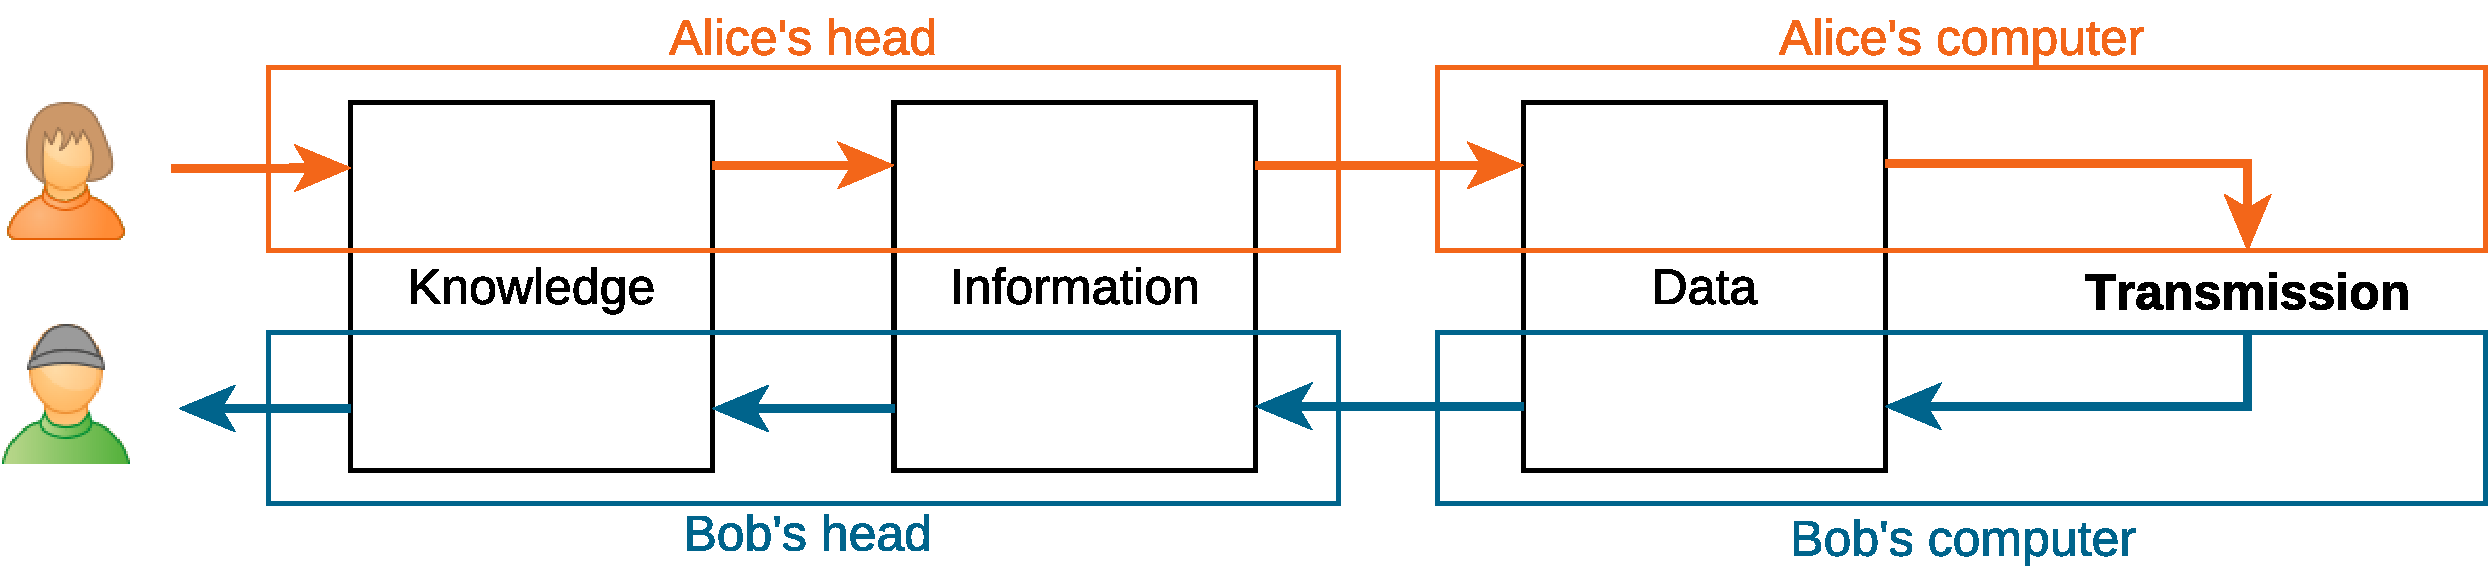
\includegraphics[width=\linewidth]{knowledge_info_data_transmission.pdf}
\end{center}

Computers work with and transmit digital \concept{data}, \ie, sequences of \concept{binary}
\zero\ and \one\ \conceptRef{symbol}{symbols}. 
However, data \concept{transmission} happens in the real world, where \zero\ and \one\ are ideas and not tangible objects.

This chapter studies how those digital symbols \textit{pierce the veil}  
from the digital to the analog (physical) world on transmission, and back from analog to digital on reception.


\section{Information $\leftrightarrow$ Data $\leftrightarrow$ Binary messages}\label{sec:piercing:information_binary}

Knowledge, \conceptRef{information}{information}, and \concept{data} are not the same thing, 
although they are often used used interchangeably. In technical contexts, they should be used and interpreted accurately.
% 
\begin{exercise}
Suppose we are outdoors and we want to tell our friend about the weather.
% 
We have knowledge about everything related to the weather, because we are there.
For our communication, we need to focus on part of that knowledge, and decide what information to send.
For instance, we could want to communicate the temperature, and say something like ``the temperature is about 22ºC''.
% 
There are many ways in which we can store that information as data inside a computer. Most likely, we will represent the number 
$22$ as part of those data. How would you define knowledge, information and data?
\end{exercise}


Even though there are many types of data, \ie\ numerical, textual, visual, scientific, \etc, these are eventually
represented by numbers. For instance, one could use \concept{ASCII} \concept{encoding} to represent the string ``Bobby''
as the following sequence: $66, 111, 98, 98, 121$.

Inside a computer, those numbers are stored in binary registers, \eg\ in the CPU and in the RAM. 
However, there are multiple ways of representing numerical data in binary format. More specifically,
we need to pay close attention to at least the following aspects whenever reading or writing data:
\begin{itemize}
\item \concept{integer} or with decimals? 
\item \concept{bitdepth}? (\eg, 8 bits per number)
\item \conceptRef{sign}{signed} or \conceptRef{sign}{unsigned}?
\item For multibyte numbers: \concept{big endian} or \concept{little endian}?
\item For numbers with decimals: \concept{floating-point} or \concept{fixed-point}?
\end{itemize}
% 
\begin{exercise}
Explain \textbf{how to complete the second row given the first} (and vice-versa),
and what assumptions you need to make in each case.
% 
\begin{center}
\begin{tabular}{lcccccc}
\toprule
\textbf{Number} 
& $7$ 
& $2$
& $-3$
& $0.75$
& $260$
\\
\midrule
\textbf{Binary} 
& \zero\zero\one\one\one
& \zero\zero\zero\zero\zero\zero\one\zero
& \one\one\zero\one
& \one\one\zero\zero
& \zero\zero\zero\zero\ \zero\one\zero\zero\ \zero\zero\zero\zero\ \zero\zero\zero\one\
\\
\bottomrule
\end{tabular}
\end{center}
% 
How about à $\leftrightarrow$ \one\one\zero\zero\ \zero\zero\one\one\ \one\zero\one\zero\ \zero\zero\zero\zero?
\end{exercise}


Sometimes we need to inspect the contents of a binary register 
(\eg, for debugging or other analysis purposes) or to set those contents manually.
% 
For humans, it is inconvenient and \textit{very} prone to error 
to handle binary strings longer than a few bits. 
When we need to inspect or modify the contents of a binary register
(\eg, for debugging purposes), we often use base $16$, \ie, \concept{hexadecimal} notation.


In hexadecimal, there are exactly $16 = 2^4$ different digits (\otherBase{0} to \otherBase{9}, \otherBase{a} to \otherBase{f})
with decimal values from $0$ to $15$, each of which represents exactly $4$ bits.
When we writing hexadecimal values to a computer, \ie, in source code, hexadecimal values are
typically preceded by \otherBase{0x}, \eg, \otherBase{0x58a5b0}. 
Similarly, binary expressions are preceded by \otherBase{0b}, \eg, \otherBase{0b0011}.

\begin{remark}
\begin{minipage}{\linewidth}
\begin{itemize}[leftmargin=0.5cm]
\item Spaces and even line breaks between digits do not carry any meaning, they are only used 
to facilitate visual inspection.
% 
\item In some texts, when multiple bases are applicable in a context, they are shown
as subscripts as in \otherBase{58a5b0$_\textrm{16}$} and \otherBase{0011$_\textrm{2}$}.
\end{itemize}
\end{minipage}
\end{remark}

\begin{exercise}
Consider the following message, which is composed of a \concept{concatenation} 
of 3-bit unsigned integers: \otherBase{a4 3f 20}.
\begin{itemize}
\item How many bits and bytes long is it?
\item\textbf{What are the first five integers} contained in the message?
\end{itemize}
\end{exercise}

Most often, we will let our code handle data manipulation. To do that, we need
\concept{bitwise} and \concept{boolean logic} operations such as the following

\begin{center}
\begin{tabular}{rcccccc}
\toprule
\textbf{Operation} & 
\conceptRef{bitwise}{bitwise AND} &
\conceptRef{boolean logic}{logic AND} &
\conceptRef{bitwise}{bitwise OR} &
\conceptRef{boolean logic}{logic OR} &
\conceptRef{bitwise}{left shift} &  
\conceptRef{bitwise}{right shift}
\\
\textbf{Python}    &
\inlineCode{&}       & 
\inlineCode{and}    & 
\inlineCode{|}       & 
\inlineCode{or}    & 
\inlineCode{<<} &  
\inlineCode{>>} 
\\
\bottomrule
\end{tabular}
\end{center}

Other useful python tools are the \texttt{bin()} and \texttt{hex()} functions, that convert an integer 
into its binary and hexadecimal representation, respectively, and \texttt{int()}, which can parse
a string describing a number and return that number. We can also control the format in which we show numbers,
\eg, \inlineCode{print(f'{n:08b}')} would print the value of variable \inlineCode{n} in binary form, 
using at least 8 positions and filling the empty leading positions with zeros
(more in the \href{https://docs.python.org/3/reference/lexical_analysis.html#f-strings}{python docs}).

\begin{exercise}
Consider the code shown next. The numbers printed when run are of special importance in networking and computer science.
What do they have in common? (Hint: You may want to modify the code to show their binary representations).

\begin{center}
\showCode{snippets/bitwisemanipulation.py}
\end{center}
\label{ex:bitwisemanipulation}
\end{exercise}
\begin{remark}
For code listings like the one above, you can download the source code and its output.
\end{remark}


\section{Analog $\leftrightarrow$ Digital}\label{sec:piercing:analog_digital}

Once we decide what bits to transmit, we need to find a way of making those bits available to another machine at a distance.
First, we need to decide what \concept{medium} to use and what physical properties we can control and monitor.
Popular choices include using voltage on \conceptRef{copper wire}{copper wires}, sending light over \concept{optical fiber} and manipulating the 
electromagnetic \concept{field} using \conceptRef{antenna}{antennas}.

\begin{exercise} \textbf{Ponder}:\\[-0.5cm]
\begin{itemize}
\item Can we make a copper cable as long as we desire?
\item What medium do Wi-Fi connexions use? 
\item Do we need optical fibers to perform light-based communication?
\end{itemize}
\end{exercise}


If we opt for copper wires, we can put several in \concept{parallel} and send more data at the same \concept{clock} speed.
This, however, comes at the price of additional complexity and cost than \concept{serial} designs. 
Voltage interferences in the \conceptRef{data line}{data lines} may happen for a number of reasons, 
including physical phenomena such as electromagnetic induction in the wire. 
Notwithstanding, cables compliant with modern data transmission standards (\eg, IEEE 802.3)
often employ \conceptRef{twisted pair}{twisted pairs of cables} and shielding
among other strategies to guarantee bit errors below $1$~in~$10^{12}$ bits.

\begin{exercise}\label{ex:piercing:copper_connectors}
\textbf{Consider and identify} the following wire connectors:\\[-0.5cm]
\begin{center}
\includegraphics[height=3cm]{hdmi_connector.jpg}
\includegraphics[height=3cm]{coaxial_connector.jpg}
\includegraphics[height=3cm]{usbc_connector.jpg}
\includegraphics[height=3cm]{rj11_connector.jpg}
\end{center}
\end{exercise}

\begin{wrapfigure}{L}{0.22\linewidth}
\includegraphics[width=\linewidth]{iceberg.jpg}
\end{wrapfigure}
Have you ever been diving in a swimming pool, looked up and the water was mirror-like?
Optical fiber cables work of this phenomenon, called \concept{refraction}.
Light that enters the fiber through one end 
stays inside until it exits through the other end. The coating of the fiber is important
to support its integrity, but that coating does not participate in the ``bouncing'' of 
light when advancing through the fiber.

In a \conceptRef{single-mode optical fiber}{single-mode} optical fiber, the sensor at the receiving end 
detects the presence or absence of a single wavelength range. These cables are relatively thin and cheap,
but carry a single signal.
% 
Another option is to transmit multiple wavelengths (\eg, using several laser sources) at the same time, 
through the same fiber. At the receiving end, a prism is used to divide the beam of light back into its
\concept{monochrome} components, which are sensed separately. 
In this way, \conceptRef{multimodal}{multi-modal optical fiber} optical fiber allows \concept{multiplexing}
several signals, greatly increasing the effective transmission rate.


\begin{exercise}\label{ex:piercing:laser_refraction}
When a beam of light enters an optical fiber, it does so with a certain angle of attack.
This angle affects the time it takes to reach the other end. If we project a cone of light,
light enters the fiber at multiple angles of attack. 
What happens at the other end if we \textbf{turn this cone of light on and off} very quickly?
Is it relevant whether we use monomodal or multimodal beams?
% 
\begin{center}
\includegraphics[height=2.5cm]{laser_refraction.jpg}
\includegraphics[height=2.5cm]{optical_connector.jpg}
\end{center}
\end{exercise}
\newpage

\begin{wrapfigure}{R}{0.3\linewidth}
\begin{center}
\includegraphics[width=\linewidth]{dipole.png}
\end{center}
\end{wrapfigure}

Even though there are many classes of \conceptRef{antenna}{antennas}, their main purpose 
is to detect electromagnetic fields and/or to create them. The Maxwell-Faraday equation tells us
that \textit{changes} in the electric \conceptRef{field (physics)}{field} $\vec{E}$ create a perpendicular magnetic \conceptRef{field (physics)}{field} $\vec{B}$,
and the other way around.

A \concept{dipole} antenna like the one to the right uses this concept by applying an alternating voltage $V$,
which generates electromagnetic waves that propagate outwards the dipole axis. 

\begin{remark}
When we emit some energy $E$ from a point in all directions, that energy is distributed around a growing sphere.
Since the area of a sphere of radius $r$ is $4 \pi r^2$, the amount of energy that reaches a point at distance $r$
will be in the \concept{ballpark} of $E / r^2$.

This is sometimes referred to as the inverse square law, and is
the reason why currents inducted in the receiver's antenna are usually between nanovols 
($10^{-9}$~V) and picovolts ($10^{-12}$~V). Surprisingly, this is enough for modern detectors to read the data signal.
\end{remark}


\begin{wrapfigure}{R}{0.2\linewidth}
 \includegraphics[width=\linewidth]{modulation.jpg}
\end{wrapfigure}


Regardless of the method chosen to let the data travel, the veil between analog signals and digital data must still be 
pierced. Once way of doing this is \concept{modulation}: a base sinusoidal signal called \concept{carrier} is produced,
and the data are encoded by modifying this carrier. For instance, once can change the \concept{amplitude} of the carrier (ASK),
its \concept{frequency} (FSK), or even the amplitude and the \concept{phase} at the same time (QAM). 

\begin{exercise}
The figure above displays an example of amplitude modulation and of frequency modulation. 
Which is which? For each case: is that \textbf{modulation transmitting an analog or a digital signal}?
\end{exercise}


\begin{exercise}
What's the \textbf{difference between bandwidth and transmission speed}? 
Why do you think they are interchangeably used in non-technical contexts?
\end{exercise}

\chapterimage{street_plaque.jpg}

\chapter{Where are you?}\label{sec:where}

Connecting two computers makes them much more useful than two isolated machines. 
However, their true potential is only unlocked when they can be connected to \textit{lots} of other computers.

Practical limitations including cost and geographic location make it impossible to directly
connect every pair of computers. Instead, devices are distributed across a graph of interconnected networks,
which may extend even beyond the scale of a planet.

Whether locally within physical reach or in another continent, an addressing system is needed
to identify, locate and route messages so that they reach their intended peers, just like we 
do with physical locations.



\section{Please contact me}\label{sec:where:topology}

When only $2$ \conceptRef{device}{devices} are involved, one may use a \concept{point-to-point} connection. In this type of connection,
there is only ``this side'' and ``the other side'' of the cable. Moreover, when a device wants to communicate with the other end, 
there is only one link (\eg, one cable) to choose from, so there is no possible confusion. Since we can operate this connection 
with just $2$ \conceptRef{network card}{network cards} and $1$ cable, point-to-point connections are viable for $N=2$ devices.

\begin{wrapfigure}{R}{0.25\linewidth}
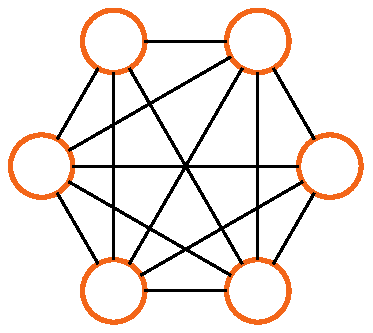
\includegraphics[width=\linewidth]{complete_graph.pdf}
\end{wrapfigure}


If we want to connect $N > 2$ devices, a naïve option is to connect every device with each other
in a \conceptRef{complete graph}{\textit{complete graph}}. Now every device needs to handle $N - 1$ cables to the other devices, 
but communicating with any other device is as easy as choosing the correct cable and establishing a point-to-point connection.

The main issue with this approach is that the total number of connections is $N \cdot (N-1) / 2 = O(N^2)$
(more on that in your trusted \textit{Discrete Math} course). This means that, in order to have $N=10$ devices connected in this way,
you would need for instance $40$ cables \textit{and} $90$ \conceptRef{network card}{network cards}. For $N=1000$ devices, 
there would be half a million point-to-point connections, which is already quite unmanageable.

\begin{remark}
$O(N^2)$ is notation for a \concept{quadratic} complexity bound. 
This is \textit{not} the same as \concept{exponential} and should never be confused.
% 
\readMore{https://en.wikipedia.org/wiki/Big_O_notation}
\end{remark}

\begin{wrapfigure}{L}{0.17\linewidth}
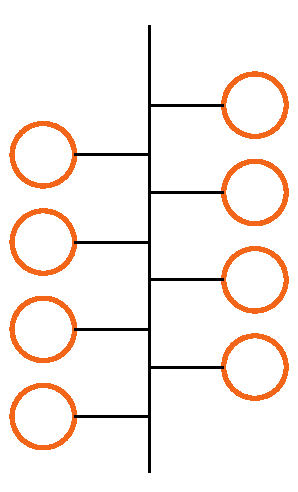
\includegraphics[height=4cm]{bus_graph.pdf}
\end{wrapfigure}

There is one trick up our sleeves: \conceptRef{bus}{data buses}, where one or more data lines
that are simultaneously connected to multiple devices. 
This retains the simplicity of point-to-point connections, because each device needs to handle
only $1$ cable and can use it to communicate with all other devices. The cost-effectiveness is 
also retained, since only $N$ network cards for $N$ devices ($O(N)$). 

The main advantage of data buses is also their main weakness: 
all devices send and receive data using the same data line, 
but they cannot do it at the same time because there is only one line. If two or more do, there is
a \concept{collision} that makes data transmission impossible while it lasts.\\[-0.5cm]

\begin{remark}
As computer networking was developed, people experimented with many alternatives to the 
bus \concept{topology}. One curious example is \concept{Token Ring}, where devices
are connected around a circle, and messages are passed around in a single direction.
\end{remark}

In practice, it is not trivial to implement a bus technology 
where new devices can be added over time. 
% 
Historically, this was sometimes done by physically piercing the main bus cable,
and adding a new cable towards the new computer being connected. 
Later on, this was simplified with devices called \conceptRef{hub}{hubs}. 
They worked similarly, but they offered pre-built \conceptRef{port (physical layer)}{ports} 
and removable connectors.
% 
Nowadays, hubs have been replaced by \conceptRef{switch}{switches}. 
Switches offer the functionality of a bus, connecting every device with each other,
and also prevent collisions. For obvious reasons, structuring connections 
around a switch is called a \concept{star topology}.

\begin{exercise}
What is \textbf{needed in a switch} that is not needed in a hub?

\begin{center}
\includegraphics[width=0.75\linewidth]{switch.jpg}
\end{center}
\end{exercise}

Bus topologies work great at local scales, and are extensively employed in
\conceptRef{LAN}{local area \conceptRef{network}{networks} (LANs)}. However, it is not cost-effective,
(sometimes not even physically possible) when devices are far apart.
% 
Instead, devices can be organized in separate LANs, each one conceptually a bus, 
and then these separate LANs can be connected using cheaper, feasible point-to-point
connections. Considered together, these devices would then form a 
\conceptRef{WAN}{wide-area network (WAN)}.

\begin{center}
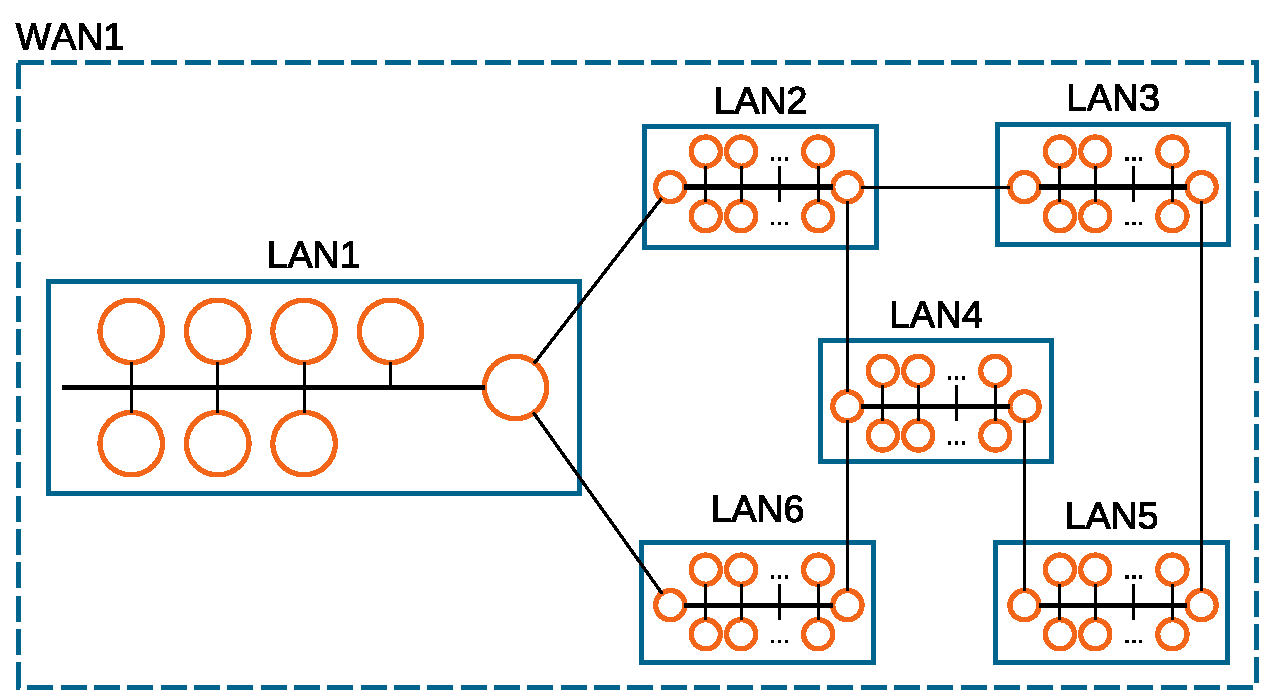
\includegraphics[width=0.65\linewidth]{lan_wan_structure.pdf}
\end{center}


\section{I need to find you}\label{sec:where:addresses}

Once again, the main advantage of data \conceptRef{bus}{buses} is also their main weakness: 
all devices send and receive data using the same data line. 
Even if collisions don't happen, every message sent into the bus is 
received by all devices.
However, what we actually want is for our message to reach its destination, 
and only its destination. Let's call this the \textit{find-my-device problem}.

The find-my-device problem is not unique of buses or \conceptRef{LAN}{LANs}. On the contrary, it becomes 
very important when we consider \conceptRef{WAN}{WANs}, where not all devices are directly interconnected.
In this case, we need to make sure we can \conceptRef{routing}{route} our messages
between different LANs, and that they reach their destination.

Surprisingly, not even point-to-point connections are safe from the find-my-device problem.
Assuming devices A and B are connected that way, two different programs may want to 
exchange information at the same time, \eg, some alarm control software and 
a music streaming app. 
In this scenario, you want the \concept{client} and \concept{server} of the alarm monitoring 
\concept{service} to communicate with each other but not with the music streaming service, 
and vice-versa.

The most common solution to this problem is to use identifiers that let
us differentiate between devices or even between running \conceptRef{process}{processes}
inside an \conceptRef{OS}{operating system (OS)}. Some of these identifiers are
referred to as \conceptRef{address}{addresses}, precisely because they are used 
to find and reach a remote device. 


\conceptRef{address}{Addresses} are typically \textit{numerical} identifiers, that is, just a number.
As such, they can be expressed in different bases, including decimal and \concept{hexadecimal}.
These numbers are drawn from a predefined set, and the choice of that set
determines the maximum number of elements we can uniquely identify.

\begin{remark}
Addresses expressed as \otherBase{d8:43:ae:61:ed:f1} or \otherBase{192.168.1.1} 
(as it will be seen later in the course) are also numbers we could have expressed 
as \otherBase{237785200061937} and \otherBase{3232235777}, respectively
(which is not as convenient).
\end{remark}

\begin{exercise}
\textbf{How many elements can be uniquely identify} (at most) with an address we express 
using 5 bits? How about 10? How about 20? Express the general solution mathematically.
\end{exercise}

\begin{exercise}
Suppose there are $1000$~machines in a LAN. \textbf{How many address bits are needed}?
How about $800$~machines? And $1100$? Express the general solution mathematically.
\end{exercise} 

\begin{remark}
In 2019, we run out of Internet (v4) addresses. Whoops!
\end{remark}

\section{How do I get there?}

In many scenarios, multiple addresses are needed to perform the desired 
\concept{end-to-end} communication. For instance, we may need to identify
a single device within a \concept{LAN}, and that LAN within a \concept{WAN}. Sometimes, we will need 
to identify a \concept{process} (a running program) within that device. 
This is not unlike someone paying you a visit in person:

\begin{minipage}{0.5\linewidth}
\begin{center}
\begin{bytefield}{16}
\bitbox{16}{Joseph Edgar Foreman} \\
\bitbox{16}{123 South Fake St.} \\
\bitbox{16}{Adams County} \\
\bitbox{16}{Ohio}
\end{bytefield}
\end{center}
\end{minipage}
% 
\begin{minipage}{0.5\linewidth}
\begin{center}
\begin{bytefield}{24}
\bitbox{24}{Process \#1717403} \\
\bitbox{24}{Device \#51688798} \\
\bitbox{24}{LAN 3141 (Data Engineering Labs)} \\
\bitbox{24}{WAN 442 (UAB)}
\end{bytefield} 
\end{center}
\end{minipage}

Whatever addressing system we use, it must contain enough information to locate and reach 
the destination, \ie, to \conceptRef{routing}{route} our messages through the graph of 
connections. The process of routing involves multiple steps or ``jumps'' across networks
until the destination LAN is reached.

The name \concept{router} refers to a type of network device
whose job is to forward these messages across networks. These devices must contain
enough information so that, when handed a message with a destination \concept{address},
they can decide what \concept{network interface} to use. 
In turn, non-router devices only need to be configured so that they can reach the next router.


\begin{remark}
At home, your \concept{router} typically also plays the role of a \concept{switch}, but those are different concepts.
\end{remark}

% \begin{center}
% 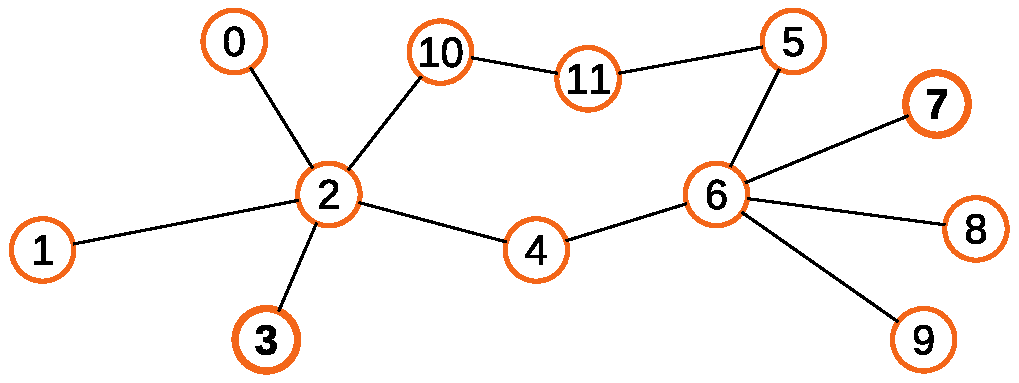
\includegraphics[width=0.5\linewidth]{how_many_packets.pdf}
% \end{center}

\begin{exercise}
This figure represents a handful of devices and their physical connections.
These devices can communicate only by sending messages through 
those connections. Notwithstanding, \node{3} wants to send a message to \node{7}.\\
% 
\begin{center}
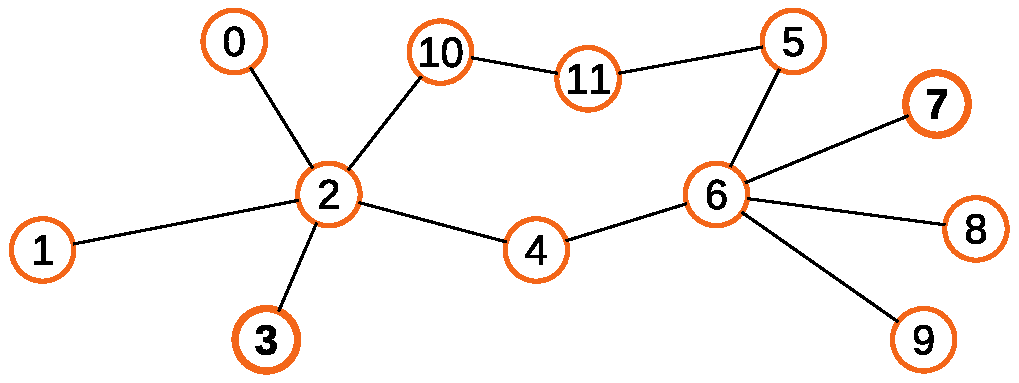
\includegraphics[width=0.5\linewidth]{how_many_packets.pdf}\\
\end{center}
% 
\begin{itemize}
 \item Can you identify any devices likely to be acting as a \concept{switch}? And as a \concept{router}?
 \item What's the \textbf{minimum number of messages} sent so that \node{3} can contact \node{7},
 and \node{7} can reply to \node{3}? List them in the order they are produced.
 \item What information needs to be included in those messages so that the communication 
 \node{3} $\leftrightarrow$ \node{7} may take place?
\end{itemize}
\label{ex:how_many_packets}
\end{exercise}
% 

\conceptRef{swimlane plot}{Swimlane plots} like the one below are used to represent the interactions
(\eg, message exchange) between actors (\eg, network devices). In them, the vertical axis represents 
time, which is invaluable to identify cause-effect relations.
\begin{center}
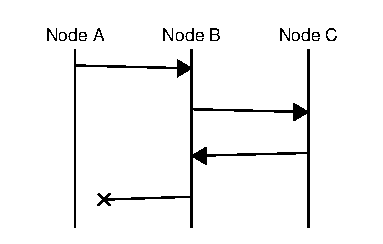
\includegraphics[width=0.35\linewidth]{swimlane_example.eps}
\end{center}

\begin{exercise}
Based on your answer to Ex.\ref{ex:how_many_packets}, \textbf{produce a swimlane diagram}
that represents the message exchanges. For each message (\eg, above the arrows), 
include the addressing information present in it.
\end{exercise}


\chapterimage{container.jpg}

\chapter{Is this yours?}\label{sec:packets}

Information travels through this graph of networks in the form of packets, which contain a small amount of 
information and meta-information. 

Packet format must be agreed upon by both ends of the communication, so that those packets can be efficiently 
and automatically produced and interpreted.

When packets travel through one or more networks, they can get lost or reordered. If a continuous stream of data must 
flow between two computers, packets must contain mechanisms to detect losses and restore the proper order.

\section{I have a delivery for you}\label{sec:packets:lan_wan}

It is not feasible to establish physical connections between each pair of computers that want to communicate.
Instead, relatively few connections are shared to carry messages between many pairs of devices.

If a single device transmits data continuously for a long time, that connection is blocked and may become a bottleneck that 
prevents other devices to communicate. To avoid this problem, connections limit the maximum amount of data
that can be sent without interruption. As a result, devices are forced to send data in discrete bursts called 
\conceptRef{packet}{packets}. The exchange of these type of messages across one or more networks is called
\concept{packet switching}.

\begin{remark}
% The concept of \concept{packet switching} (crucial to the creation of the Internet)
% was developed in the 1960's (during the cold war) by the US military
% to have a communications network that would work in case of a nuclear strike.
%  
% The problem with the one they had was that, if one station was damaged, the whole system stopped working.
% However, by using packet switching, any connected subgraph of the network would keep working.
% 
% The reasoning for creating a packet-switched network was that they could still retaliate their enemy in case of an attack, which would
% make them a less attractive target.

Leonard Kleinrock, one of the pioneers of internetworking, disputes the authorship of packet switching,
which is often attributed to Paul Baran and Donald Davies.
\end{remark}

\conceptRef{packet}{Packets} need to be small so that connections are not blocked for too long. 
At the same time, we want packets to contain as much data as possible, because each packets 
contain \concept{overhead} data (such as the addresses discussed in Section~\ref{sec:where}) that need
to be sent in addition to the user's payload data. Networks set the maximum packet length
using a parameter called \conceptRef{MTU}{Maximum Transmission Unit} (MTU), \eg, 1500~bytes in Ethernet.


Packet transmission across a \concept{data link} must be done carefully,
particularly when that link is a \concept{bus} shared by multiple devices.
Each packet must be individually distinguishable from the rest, 
which can be done via at least three strategies:
\begin{enumerate}
\item \textit{Fixed length}: the length of all packets is the same. The sender and the receiver must have
agreed to this value in advance.

\item \textit{Explicit length}: the length of the packet is included in the packet, \eg, 
using the first byte of the packet. The sender and the receiver must agree on how this information
is included and how to interpret it.

\item \textit{Escape sequences}: Certain binary \conceptRef{escape sequence}{escape sequences} 
within the data have a special meaning. 
For instance, one could define the byte \otherBase{11110000} (\otherBase{0xf0}) 
to mean ``end of packet'': these bits must appear after each packet, and only then.
% 
Then the sender could start transmitting the contents of a packet, followed by \otherBase{0xf0}.
Both parties must agree on what escape sequences to use, what they mean, and how to 
send data equal to those sequences (\eg, it should be possible to send \otherBase{0xf0f0f0}
without triggering an ``end of packet'' until all bytes are transmitted).
\end{enumerate}

\begin{remark}
It is also possible to to signal the \textit{beginning} of a packet. In that case, a preceding sequence called \concept{preamble} is used.
\end{remark}


\begin{exercise}
All strategies described above are used nowadays in real scenarios, depending on the 
features, costs and trade-offs of each one.

Discuss which of these strategies would be most appropriate for each of these scenarios:
\begin{itemize}
\item A single manufacturer designs the hardware and software that communicates two endpoints.
A single \concept{data line} must be \conceptRef{multiplex}{multiplexed} for multiple control commands
as well as multiple data streams. The priority is efficient power and buffer usage.

\item Multiple devices share a \concept{bus}. They occasionally send messages of different lengths,
but not a huge volume of data. The priority is cost.

\item Multiple devices share a \concept{bus}. They continuously send messages of different lengths,
trying to maximize the effective transmission rate through the \concept{channel}. 
The priority is \concept{throughput}.
\end{itemize}
\end{exercise}

\section{Please fill in the form}\label{sec:packets:format}

Regardless of the strategy employed, data packets typically comprise two parts: 
\begin{itemize}
 \item Data \concept{payload}: the information that needs to be transmitted, and
 \item \conceptRef{metadata}{Metadata}: the meta-information needed to deliver the payload.
\end{itemize}
Length might be one of the metadata \conceptRef{field (packet)}{fields} included in the packet, along with 
others that help identify their type and function.
% 
The location of payload and metadata, as well as the exact metadata fields included, their length and their meaning
must be known by both ends of the communication. All these decisions constitute the \concept{packet format}
or \concept{packet structure}.

One of the most common ways of arranging payload and metadata is with a \concept{header}-\concept{body} format.
In this case, all meta-information is included first, followed by the data. 
Other formats may include a \concept{trailer} (also known as \concept{tail}, most often used for \concept{error detection}
and correction), in combination with the header, or replacing it.
All of the following configurations are possible.

\begin{minipage}{\linewidth}
\begin{center}
\begin{bytefield}{32}
\bitbox{11}{Header} & \bitbox{21}{Body}\\[-0.35cm]
\end{bytefield}
% 
\begin{bytefield}{32}
\bitbox{6}{Header} & \bitbox{19}{Body} & \bitbox{7}{Trailer/Tail}\\[-0.35cm]
\end{bytefield}
% 
\begin{bytefield}{32}
\bitbox{21}{Body} & \bitbox{11}{Trailer/Tail}\\[-0.35cm]
\end{bytefield}
% 
\begin{bytefield}{32}
\bitbox{32}{Header}
\end{bytefield}
\end{center}
\end{minipage}


The format of the payload in a packet is normally user-defined. The format of the header, however,
is strictly defined so that it can be easily produced and \conceptRef{parsing}{parsed}.
This format is often presented using a diagram that helps identify the individual bit and byte positions,
like in the following (not-real) example:\\

\begin{center}
\begin{bytefield}{32}
\bitheader{0-31} \\
\begin{rightwordgroup}{Header}
\bitbox{16}{Length} & \bitbox{8}{Importance} & \bitbox{4}{Type} & \bitbox{4}{Mode}\\
\bitbox{24}{Destination Address} & \bitbox{8}{(Reserved)} 
\end{rightwordgroup} \\
\begin{rightwordgroup}{Body}
\wordbox[lrt]{1}{Payload} \\
\skippedwords \\
\wordbox[lrb]{1}{} 
\end{rightwordgroup}
\end{bytefield}
\end{center}

\begin{remark}
Fields may also have fixed or variable lengths, which do not necessarily align with 
\conceptRef{byte boundary}{byte boundaries}. Fields may also have length equal to $1$~bit,
in which case its is normally called a \concept{flag} or flag bit.d
\end{remark}


\begin{remark}
In diagrams like the one above, multiple lines (rows) are often used so that they can be
easily printed and read. In that case, the meaning is the same as if all fields had been
presented along the same line (row).
\end{remark}

\begin{exercise}
The following packet contents were \conceptRef{sniff}{sniffed} out of a \concept{network},
expressed in \concept{hexadecimal}. Assuming the packet has the format of the example above:
% 
\begin{itemize}
\item Indicate the value of each field (length, importance, type, mode, destination address, and payload.
\item Can you guess the meaning of the payload?
\end{itemize}
% 
\begin{center}
\otherBase{00 0c 00 f3 bb bb bb 00 68 65 6c 70}
\end{center}
\end{exercise}

\begin{exercise}
The following code accepts two arguments: (1, \inlineCode{sys.argv[1]}) the \concept{path} of an input file, 
and (2, \inlineCode{sys.argv[2]}) the \concept{path} of an output file.
The first 255 bytes of the contents of the input file are read, 
they are formatted as a packet, and the bytes of that packet
are output to the output file.

\begin{center}
\showCode{snippets/simplepacketoutput.py}
\end{center}

\begin{itemize}
\item Describe the \concept{packet format} used in the code, and its limitations.

\item Extend the packet format so that 
 \begin{itemize}
   \item Packets can be longer than 255 bytes
   \item The \concept{address} of the destination device can be encoded
  \end{itemize}
  
\item Provide a byte diagram of the new format, 
as well as an explanation of the addressing system you are using.

\item Modify the code so that it outputs packets of your proposed format.
\end{itemize}
\end{exercise}

\begin{remark}
Languages like Python can make a distinction between files containing text and files containing binary data.
In the code above, files are open in \concept{binary mode} using modes \inlineCode{'rb'} and \inlineCode{'wb'}.

When open in binary mode, file bytes are directly represented by a \inlineCode{bytes} object, an array of 
integers between $0$ and $255$. In \concept{text mode}, those bytes are processed (\conceptRef{decode}{decoded}) further by the \inlineCode{open} method,
and returns a string that might contain special characters like accents or non-latin glyphs. \readMore{https://docs.python.org/3.12/library/functions.html\#open}
\end{remark}

\section{They keep coming}\label{sec:packets:stream}

When developing applications that use networking capabilities, it is often useful 
to imagine communication as a \concept{stream}, \ie, as a conceptual pipe where we put 
our data (any amount of data) in one end, and it comes out at the other end. If we have
this capability, then it becomes much easier to send files of any size, and to transmit a never-ending
amount of audio or video. Unfortunately, all we have to simulate those streams are packets.

\conceptRef{packet}{Packets} often need to be forwarded through multiple networks. \conceptRef{router}{Routers} are not perfect
and are sometimes inoperative or improperly configured, so not all packets arrive to their destination. Moreover,
different packets may be delivered through different routes that may be of different length, so packets may arrive
out of order.

If we want to simulate a \concept{stream} of data, packets must contain enough meta-information in them so that losses can be detected and 
the correct order can be restored. This introduces an \concept{overhead} that is not suitable in all scenarios --\eg, very low latency--,
so some applications base their network communication in \conceptRef{message}{messages} instead of streams.

When streams are required, the concept of \concept{offset} is used to reassemble multiple messages into 
a single stream. Each packet contains some bytes of the data stream, and the offset indicates the exact location in that stream.

\begin{exercise}

The following diagram describes a stream of 48 bytes produced by a source node, 
as well as the packets it was split into before transmission:\\[-0.25cm]

\begin{center}
\begin{bytefield}[bitheight=2cm]{48}
\bitheader{0-47} \\
\bitbox{10}{\underline{Packet 0} \\Offset 0 \\Length 10}
\bitbox{14}{\underline{Packet 1} \\Offset 10\\Length 14}
\bitbox{6 }{\underline{Packet 2} \\Offset 24\\Length 6 }
\bitbox{18}{\underline{Packet 3} \\Offset 30\\Length 18}
\end{bytefield}
\end{center}

\begin{itemize}
\item Describe the minimum header that can be used to transmit this stream.
\item Assuming that the recipient receives Packet 2 first, followed by Packet 0 and other packets are lost: what bytes of the stream are known by the 
  destination node, and what bytes are unknown?
\item How can the source node know that some packets were not delivered?
\item What would happen if a bogus message is received by the destination, with offset $7$~bytes and length $4$~bytes?
\end{itemize}

\end{exercise}



\chapterimage{onions.jpg}


\chapter{A Stack of Layers}\label{sec:stack_layers}

Modern computer communication is achieved using a
\concept{stack} of network \conceptRef{layer}{layers}.
Each stack focuses on some problems and is responsible for 
providing certain features, \eg, 
\concept{addressing} and \concept{sequencing} (introduced in the previous chapters).

Each \concept{layer} defines a \inlineCode{send}/\inlineCode{receive} function \textit{pair},
which is responsible for some of these features.
% 
Each layer uses the \inlineCode{send} and \inlineCode{receive} of the layer below,
\ie, the features of one layer rely on the features of all layers below it.

To coordinate layers and enable \concept{virtual} communication between them, 
each layer defines a different \concept{packet format}, which \conceptRef{encapsulate}{encapsulates} 
a packet of the layer above it.


\section{Sending data}

To implement these 
capabilities, each layer transmits not only the \inlineCode{data} provided by the layer above, 
but also a header with all the meta-information required for that capability. Thus, each layer needs to define
the \concept{packet format}, adding some \concept{overhead} (typically a \concept{header}) to the \concept{payload}, \eg:

\begin{center}
    \begin{bytefield}{36}
     \bitbox{12}{Header} & \bitbox{24}{Payload}
    \end{bytefield}
\end{center}



When a user program wants to send some data, it uses the \inlineCode{send} method of the \textit{top} layer of the stack,
which eventually results in some data being transmitted by the physical layer, \eg, through a cable or antenna.
The following figure depicts the structure of a 4-layer \concept{stack}:

\begin{center}
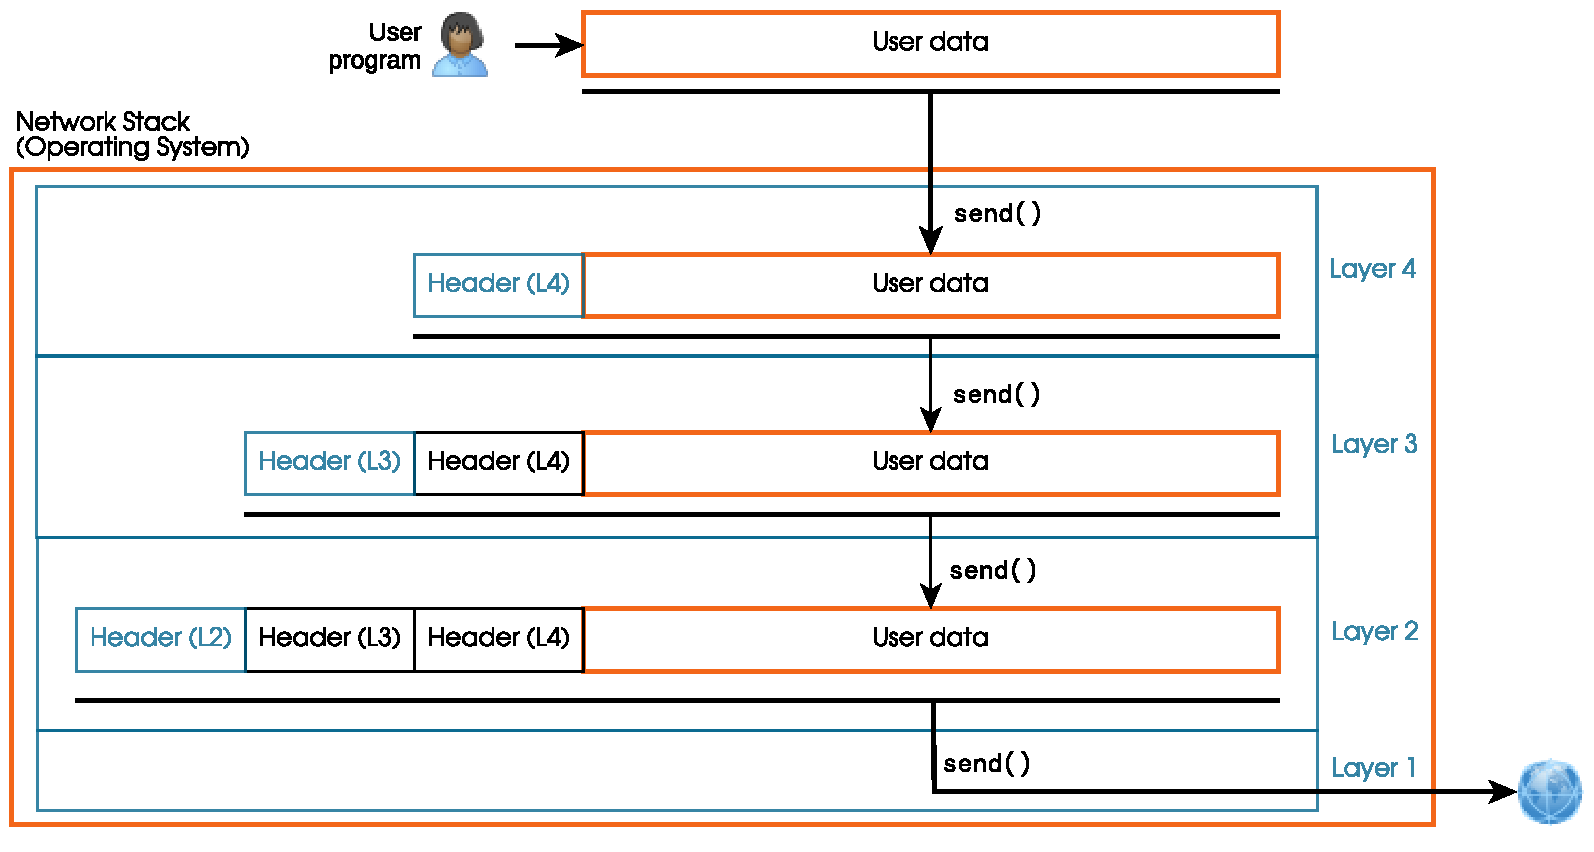
\includegraphics[width=\linewidth]{encapsulation_send.pdf}
\end{center}


The packets produced by each layer are generically referred to as \concept{PDU}s (Protocol Data Unit).
The PDUs of each layer have specific names such as \concept{frame}, \concept{datagram} or \concept{segment}.
These names must be used with precision in technical contexts.

Each layer includes the \concept{PDU} of the layer above inside its PDU's \concept{packet format} definition.
This process is referred to as \concept{encapsulation}.

\begin{exercise}

The user program wants to send $420$~bytes of data using the \concept{stack} of the previous figure.
Assume a header size for layers 2, 3 and 4 of $14$~bytes, $20$~bytes and $20$~bytes, respectively.
\begin{itemize}
    \item What is the \concept{payload} size and the \concept{overhead} size for each \concept{layer}'s \concept{PDU}?
    \item What is the \concept{payload} size and the \concept{overhead} size of the whole \concept{stack}?
\end{itemize}
\end{exercise}

\section{Receiving data}

When a \concept{packet} reaches the network \concept{stack} of the recipient, it is processed in reverse order,
\ie, layers are traversed from bottom to top. Each layer inspects \textit{only} the \concept{header} corresponding to that layer.
If everything is correct, the layer removes the header and passes the remainder of the packet to the layer above.
In turn, the layer on top passes the remaining data (the \concept{payload}) to the recipient.
Continuing the example of the 4-layer stack:

\begin{center}
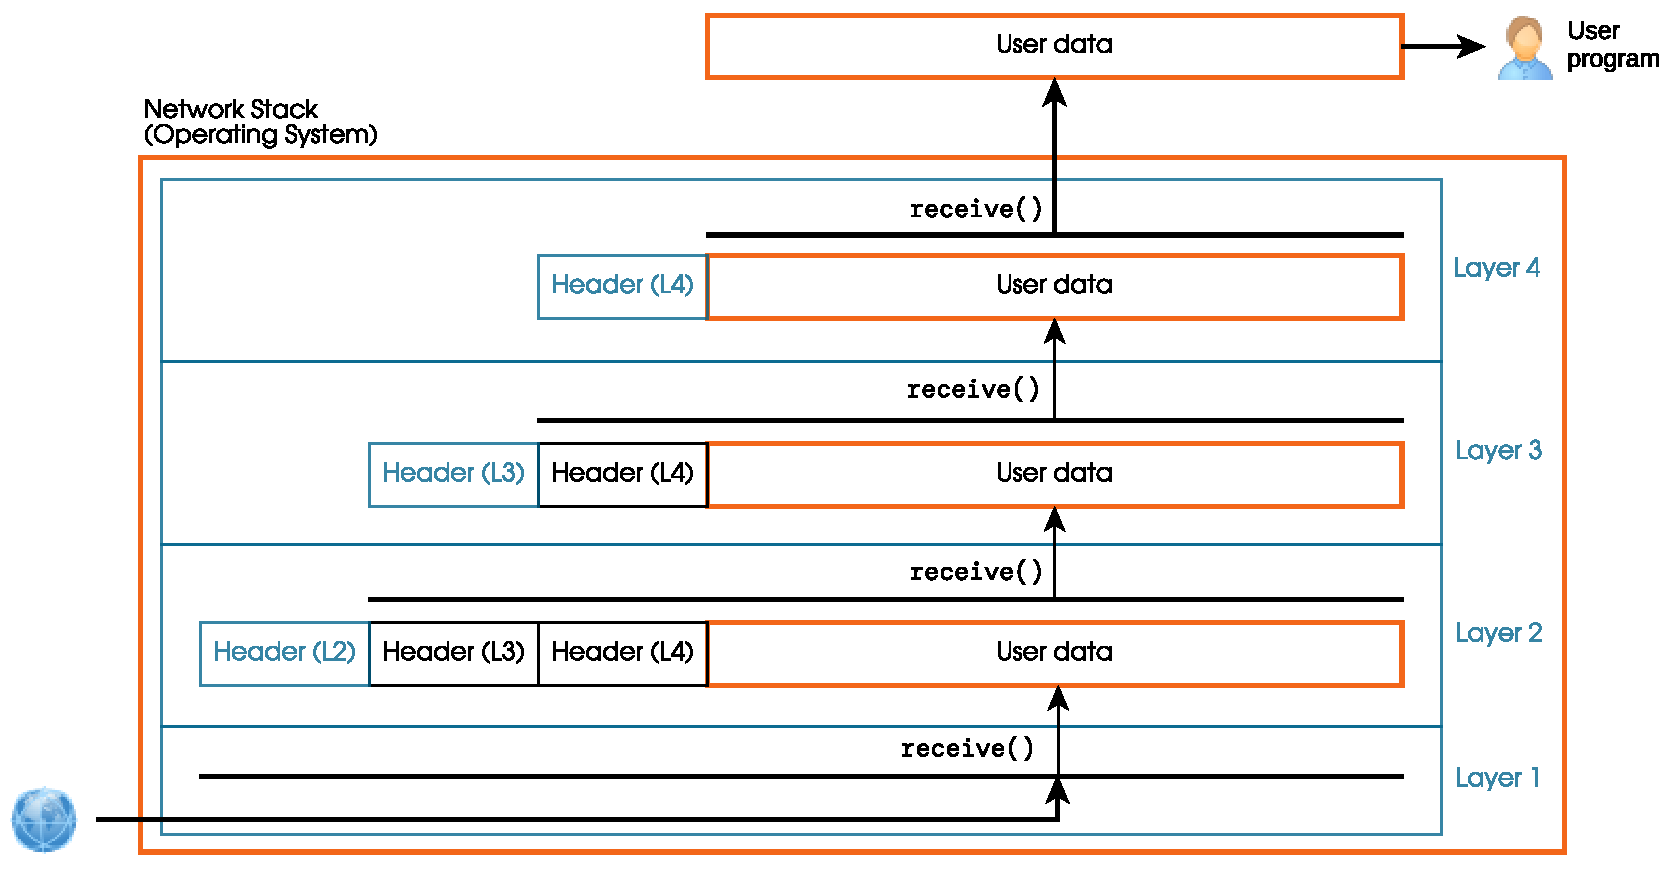
\includegraphics[width=\linewidth]{encapsulation_receive.pdf}
\end{center}


In a \conceptRef{stack}{network stack}, only the bottom layer interacts directly with the exterior,
\eg, only the physical network card of a computer is connected to a wire that carries data to other computers.
% 
At the same time, data sent by the bottom layer includes the \conceptRef{PDU}{PUDs} of all layers
by means of \concept{encapsulation}.
% 
Thanks to this, there exists a \concept{virtual} communication between each layer in one end and its counterpart in the other 
end of communication. The following figure represents the real (solid line) and virtual (dashed line) communication 
in our example:

\begin{center}
    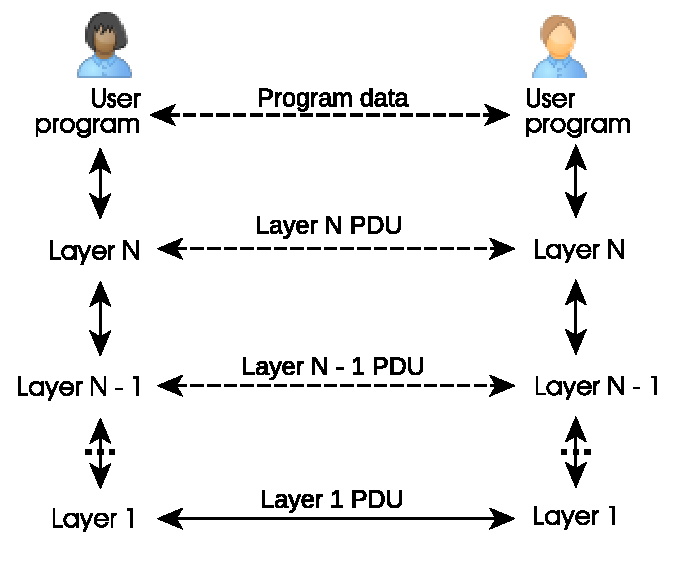
\includegraphics[width=0.5\linewidth]{horizontal_layer_communication.pdf}
\end{center}


\begin{exercise}
Another network \concept{stack} example has 3 layers: L1, L2 and L3 from bottom to top.

The \concept{PDU} of layer L2 is as follows:

\begin{center}
\begin{bytefield}{32}
\bitheader{0,7,8,15,16,23,24,31}\\
\bitbox{16}{Destination address} & \bitbox{16}{Payload length (bytes)} \\
\wordbox{2}{{Payload (variable length)\\$\vdots$}}
\end{bytefield}
\end{center}

The \concept{PDU} of layer L3 is as follows:

\begin{center}
\begin{bytefield}{32}
\bitheader{0,7,8,15,16,23,24,31}\\
\bitbox{16}{Fragment offset} & \bitbox{16}{Payload length (bytes)} \\
\wordbox{2}{{Payload (variable length)\\$\vdots$}}
\end{bytefield}
\end{center}

Layer L1 receives a \concept{packet} of data and its \inlineCode{receive} function returns the following data
(assume \concept{unsigned} integers and \concept{big endian} order when needed:
\begin{center}
\otherBase{01 23 00 0a 01 00 00 06 00 aa 00 bb 43 20}
\end{center}
\begin{itemize}
\item What data \concept{payload} was sent to the recipient program in this \concept{packet}?\\[-0.25cm]

\item If this is the last \concept{packet} of the communication, how much (\concept{payload}) data was sent
  to the recipient user program?\\[-0.25cm]
  
\item At most, how many different computers can connect using this \concept{stack}?\\[-0.25cm]

\item We send a file as the payload of this stack. What's its maximum possible size?
\end{itemize}
\label{ex:how_it_is_done:three_layer_network}
\end{exercise}

\begin{center}
\showCode{snippets/encapsulation.py}
\end{center}

\begin{exercise}
The previous code takes some data and writes the bytes that would be sent to Layer 1 
(the \concept{physical layer}) of the \concept{network stack} of Exercise~\ref{ex:how_it_is_done:three_layer_network}.
Implement the receiving end of the stack as follows: 

\begin{itemize}
\item Implement a \inlineCode{layer2_decapsulate(data: bytes) -> (int, bytes)} function that takes a Layer 2 PDU
  and returns the tuple \inlineCode{(address, payload)}, where \inlineCode{address} is the destination address and 
  \inlineCode{payload} is the encapsulated Layer 3 PDU.\\[-0.25cm]
  
\item Implement a \inlineCode{layer3_decapsulate(data: bytes) -> (int, bytes)} function that takes a Layer 3 PDU
  and returns the tuple \inlineCode{(offset, payload)}, where \inlineCode{offset} is the payload offset, and 
  \inlineCode{payload} is the chunk of data sent by the other end of communication.\\[-0.25cm]
  
\item Implement a \inlineCode{stack_receive(data: bytes)} function that decodes a Layer 1 PDU (using the two previous functions)
  and prints a message line similar to 
  \begin{center}
  \inlineCode{"Received a chunk of data. Length: 12 bytes, Address: 0xabcd, Offset: 0."}
  \end{center}\ \\[-0.75cm]
  
\item Complete the \inlineCode{stack_send} function so that the input data are split in chunks of at most 100 bytes, 
      a valid Layer 1 PDU is produced for each of those chunks,
      and those Layer 1 PDUs are passed to \inlineCode{stack_receive}.\\[-0.25cm]
      
\item Would your implementation work if the Layer 1 PDUs were randomly ordered before passing them to the receiving stack?
\end{itemize}
% 
\label{ex:how_it_is_done:implementation_three_layer_network}
\end{exercise}

\begin{remark}
Python's \inlineCode{struct} library is useful, but not mandatory, to format \concept{packet} bytes.
\end{remark}


\part{Internet}
\ \\[-10cm]
The previous part of this guide explored some of the main challenges of communicating multiple computers.
The \concept{Internet} is one working solution to those challenges: the one humans have created over the last half century,
now central to many social, commercial and political activities. 
% 
This part studies the main features offered by the Internet, as well as the \concept{suit} of \conceptRef{protocol}{protocols} 
employed to achieve them.


\chapterimage{earth.jpg}

\chapter{The Internet}\label{sec:internet}

Modern communications are based on layered network \conceptRef{stack}{stacks}. 
Maybe you just downloaded this guide from the Internet.
% 
What layers are used exactly? What protocols are employed, and with what purpose?
% 
This chapter provides a primer to answer these questions.\\[-1cm]

\section{The TCP/IP stack}


The \concept{Internet} is a practical solution to the problem of global computer communication,
whose development started in the late 1960's -- early 1970's, and is still ongoing.

\conceptRef{packet}{Packet} switching was conceived during the early 1960s, and the first 
wide-area implementation, \concept{ARPANET}, began in 1969. 
% 
A key challenge at the time was to interconnect existing \conceptRef{network}{networks}, 
owned by different organizations, and based on different technologies and \conceptRef{protocol}{protocols}.
% 
To make things viable, all the following requirements had to be met:
\begin{itemize}
    \item Existing networks should work without updates to the physical infrastructure 
      or their protocols, just the way those protocols are used.
    \item Existing networks should remain independently managed at the local level (autonomous internal organization).
    \item Packets may not always be delivered, some are lost.
    \item Messages that arrive may not be in order, and may be repeated.
\end{itemize}

The solution adopted by ARPANET --and later by the whole world-- 
is the \concept{TCP/IP} protocol suite, first described in 1974. 
It is a layered approach, designed to be ``plugged-in'' on top of 
existing \conceptRef{LAN}{LANs}, with the goal of offering networking 
capabilities to all user applications.

\begin{center}
\begin{bytefield}{16}
\begin{rightwordgroup}[curlyshrinkage=10pt]{User programs}
\wordbox{3}{Layer 7: Application}
\end{rightwordgroup} \\
\begin{rightwordgroup}[curlystyle=\color{color1},curlyshrinkage=10pt]{{\color{color1} TCP/IP}}
\wordbox{1}{Layer 4: Transport}\\
\wordbox{1}{Layer 3: Internet}
\end{rightwordgroup} \\
\begin{rightwordgroup}[curlyshrinkage=10pt]{Existing/future LAN technologies}
\wordbox{1}{Layer 2: Network}\\
\wordbox{1}{Layer 1: Physical}
\end{rightwordgroup}
\end{bytefield}
\end{center} 
 
In a nutshell, the main services offered by these layers are as follows:
\begin{enumerate}
\item[\textbf{Layer 1}] \textbf{(Physical)}: 
  Send \concept{digital} data through \concept{analog} media.
\item[\textbf{Layer 2}] \textbf{(Network)}:
  Identify and communicate devices within the same \concept{LAN}.\\
  The term ``Data Link'' layer (from the OSI model) is sometimes used.
\item[\textbf{Layer 3}] \textbf{(Internet)}:
  Identify and communicate devices across all \conceptRef{LAN}{LANs}.\\
  The term ``Network'' layer (also from OSI) is sometimes used.
\item[\textbf{Layer 4}] \textbf{(Transport)}:
  Identify and communicate programs (services).\\
  Also (choose \textit{only} one):
  \begin{enumerate}[label=\alph*)]
   \item Make sure a \concept{stream} of data successfully reaches the other end, 
   and in order \\-- \textit{but} an \concept{overhead} is introduced 
   and \conceptRef{connection}{connections} must be established (\concept{TCP}).
     
   \item Use simple, relatively efficient messages, and have a small overhead\\
   -- \textit{but} messages may be lost, reordered or duplicated (\concept{UDP}).
  \end{enumerate}
\item[\textbf{Layer 7}] \textbf{(Application)}:
  Do anything the user might need. \\
  Don't forget about security (\eg, cryptography) 
  or about efficiency (\eg, compression): Layers 4 and below don't provide that.
\end{enumerate}

\section{TCP/IP protocol overview}

Multiple \conceptRef{protocol}{protocols} are defined to implement the functionality
of each \concept{layer}. These definitions include the required \concept{packet format},
the rules to exchange those packets and their semantics.
% 
These protocols must be understood as a system, in which each part has very specific tasks.

Some of the most relevant protocols to communications using the Internet 
are shown in the next figure. In it:
\begin{itemize}
\item Solid arrows indicate a protocol being encapsulated in another. 
  If the destination is a layer, one protocol within that layer must be used.

\item Dashed boxes indicate auxiliary protocols defined to help other function. 
Dashed arrows indicate what layer uses what auxiliary protocol.

\item Boxes with thicker lines indicate the protocols highlighted in this guide.
\end{itemize}

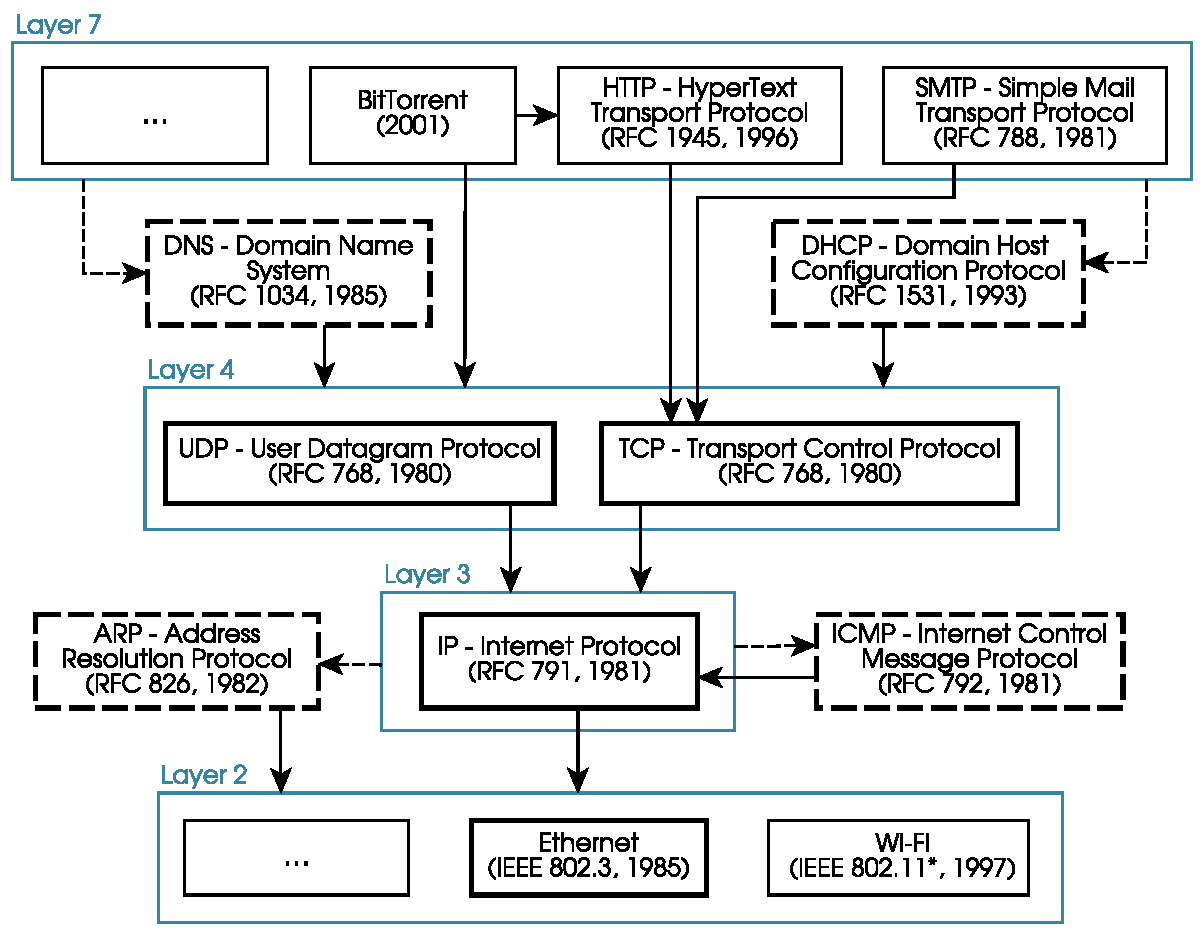
\includegraphics[width=\linewidth]{protocol_dependencies.pdf}

\begin{exercise}
We want to send the sentence ``Sorry, I'll be 5 minutes late'' by email.
Our email client will send those data using the SMTP protocol, which in turn
uses TCP (part of Layer 4).
% 
Assuming SMTP uses headers in its \concept{PDU}, how many headers will 
the corresponding Layer-2 \concept{PDU} contain?
\end{exercise}

\begin{exercise}
Why do you think Layer~3 has only one protocol (two if you count IPv4 and IPv6 separately)? 
\end{exercise}

\section{Who is the Internet boss?}

The \conceptRef{IETF}{Internet Engineering Task Force (IETF)} was created in 1986
to develop and publish standards to be used in the Internet. 
% 
Their main output are  \conceptRef{RFC}{``Request for Comment'' (RFC)} documents,
which contain complete technical descriptions of those standards.


These RFCs are created by working groups of experts, 
for everyone to use freely and free of charge. 
% 
Anyone can participate in these working groups, including researchers,
governments and industry stakeholders. 
% 
Decisions are made when 80-90\% of the participants agree, so no single 
entity controls the standardization process.
% 
\begin{remark}
``We reject kings, presidents, and voting. 
We believe in rough consensus and running code'' 
--- Dave Clark (IETF), 1992.

See DOI \href{https://dx.doi.org/10.1109/MAHC.2006.42}{\underline{10.1109/MAHC.2006.42}} for 
a short story of struggle for power.
\end{remark}

RFCs standards are descriptive, not prescriptive. This means that nobody polices the correct 
use of these standards. Instead, manufacturers have the incentive to be compliant with the RFCs 
so that their products are compatible with others. 
% 
The value of RFCs (and any other standard) is dependent on whether
they are adopted by users. RFCs can be updated and \conceptRef{retire (standard)}{retired} for this reason.

TCP/IP protocols prevail because they are flexible and work reasonably well in most situations, 
even though they are not optimal in virtually any of them. 
Also, TCP/IP protocols are free, as opposed to \concept{privative} protocols
that forced the purchase of a specific vendor's solution.
% 
\begin{remark}
Today it is hard to imagine a world \textit{not} 
dominated by the TCP/IP architecture, 
but entirely different stacks were commercialized and supported until the late 90s.
Examples include AppleTalk and IPX/SPX, by Apple and Novell, respectively.
\end{remark}

% https://www.icann.org/en/blogs/details/cheers-to-the-multistakeholder-community-30-9-2016-en

Some aspects of TCP/IP like unique identifiers 
(including \concept{DNS}, the Domain Name System)
and reserved numbers need to be agreed upon by everyone for the Internet to work properly.
% 
The \concept{IANA} (Internet Assigned Numbers Authority) works in coordination with the \concept{IETF}
to define the appropriate \conceptRef{RFC}{RFCs}.

\begin{remark}
Since 2016, IANA is managed by a nonprofit multistakeholder organization 
(\conceptRef{ICANN}{ICANN - Internet Corporation for Assigned Names and Numbers}).
% 
Since 2004, the responsibility for regional domains 
(\eg, \url{.cat}, \url{.fr}, \url{.es}) is transferred to continent-level 
organizations called regional Internet Registries (\conceptRef{RIR}{RIRs}).
\end{remark}



% # Based on https://www.youtube.com/watch?v=oIezCGjxV3A
% year,text
% 1962,Packet Switching
% 1969,ARPANET
% 1974,TCP/IP
% 1986,IETF
% 1991,WWW
% 1993,CIDR addressing
% 1998,Google
% ``The Internet doesn't do what the endpoints can do (\eg, reliability or compression).''


% - In February 1980, the Institute of Electrical and Electronics Engineers (IEEE) started project 802 to standardize local area networks (LAN).[16][27 (https://en.wikipedia.org/wiki/Ethernet)

% "protocols": "the first sheet of a volume" (on which contents and errata were written

% \begin{remark}
% Extra:
% \begin{itemize}
%     \item Video: https://www.youtube.com/watch?v=oIezCGjxV3A (part 1), https://www.youtube.com/watch?v=RN4gSBTANUY (part 2)
%     \item Monographic: https://cacm.acm.org/research/on-the-hourglass-model/
% \end{itemize}
% \end{remark}


% \begin{itemize}
% \item [\textbf{Layer 1}:] \textbf{Physical}
%     \begin{itemize}
%     \item[Features:] Ship \concept{digital} \otherBase{0}s and \otherBase{1}s through the real, \concept{analog} world.
%     \item[Offers:] Send and receive blocks of bytes.
%     \end{itemize}
% 
% \item [\textbf{Layer 2}:] \textbf{Network}\\
% 
% 
% \item [\textbf{Layer 3}:] \textbf{Internet}\\
% \item [\textbf{Layer 4}:] \textbf{Transport}\\
% \item [\textbf{Layer 7}:] \textbf{Application}\\
% \end{itemize}
% 
% \begin{remark}
% The \concept{OSI} model is a conceptual stack of layers that divides problems a bit differently from \concept{TCP/IP}. 
% TCP/IP was created on the go while the infrastructure of the Internet started its development, became its de-facto standard,
% and is used everywhere. The OSI model is useful to analyze and design communication protocols, but has limited practical usage.
% \end{remark}
% 
% 
% The network stack is normally part of the \concept{operating system} (OS).
% Only the \inlineCode{send} and \inlineCode{receive} functions of Layer 4 are exposed to the users of the OS.
% %
% This way, data transmitted by the \concept{network interface} are guaranteed to be properly formatted and follow
% the protocols of each stack layer.
% 
% \begin{remark}
% In order to control the lower layers --\eg, to transmit custom PDUs--, one needs to be the \texttt{root} user
% or give the \texttt{CAP\_NET\_RAW} kernel capability to a user program
% (or the equivalent in privative systems).
% \end{remark}
% 
% 
% \section{}\label{sec:stack_layers:organization}
% 
% - internet organization 
% bodies and stuff

\chapterimage{lan_party.jpg}
\chapter{Layer 2: Network (LAN) communication}\label{sec:layer2}

\begin{minipage}{0.4\linewidth}
\begin{center}
\begin{bytefield}{16}
\bitbox{16}{Layer 7: Application} \\
\bitbox{16}{Layer 4: Transport} \\
\bitbox{16}{Layer 3: Internet} \\
\bitbox{16}{\color{color1} Layer 2: Network (LAN)} \\
\bitbox{16}{Layer 1: Physical} \\
\end{bytefield}
\end{center}
\end{minipage}
\begin{minipage}{0.6\linewidth}
\begin{center}
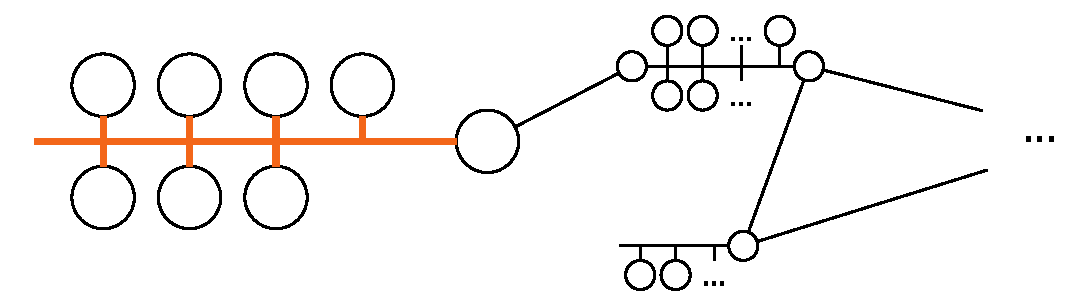
\includegraphics[width=\linewidth]{network_layer2.pdf}
\end{center}
\end{minipage}

\vspace{-0.75cm}

% \section{Layer~2 overview}
\subsection*{Capabilities}

Layer~2 protocols allow multiple devices to exchange messages
and identify each other within a local network (\concept{LAN}).
% 
Devices outside the LAN cannot be contacted \textit{directly} with Layer~2 protocols.

Layer~2 abstracts upper layers (including user applications) from the specifics of connected hardware.
This makes it easier (read: cheaper) to write code once and run it everywhere.

Layer~2 messages are limited in length. The maximum amount of Payload data 
that can be inserted in a Layer~2 protocol is called the \conceptRef{MTU}{Maximum Transmission Unit (MTU)},
\eg, $1500$~bytes for Ethernet.

Some Layer~2 protocols may also provide user \concept{authentication} and
\conceptRef{cryptography}{cryptographic} protection; 
\concept{Wi-Fi} is a notable example,
although wired networks may also employ, \eg, IEEE 802.1X.

\vspace{-0.3cm}
\begin{center}
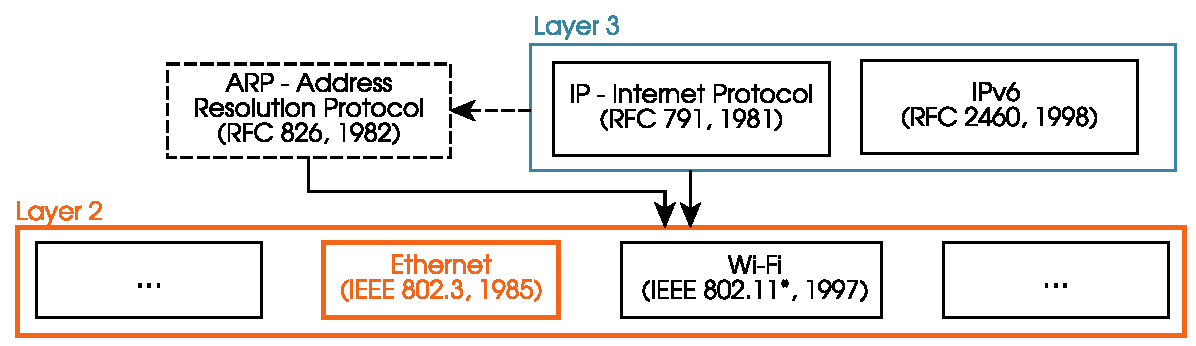
\includegraphics[width=0.9\linewidth]{protocols_layer2.pdf}
\end{center}
\vspace{-0.5cm}

\subsection*{Protocols}
Many \concept{protocols} have been and are being defined within Layer~2. Most importantly nowadays:\\[-0.65cm]
\begin{itemize}
\item \concept{Ethernet} (IEEE 802.3), addressed in \secref{sec:layer2:ethernet}.
\item \concept{Wi-Fi} (\eg, IEEE 802.11be aka Wi-Fi 7, of 2024).
\end{itemize}

Within \concept{TCP/IP}, Layer~2 \conceptRef{encapsulation}{encapsulates} the following protocol \conceptRef{PDU}{PDUs}
(both addressed in Chapter~\ref{sec:layer3}):\\[-0.65cm]
\begin{itemize}
  \item \concept{IPv4} and \concept{IPv6} \conceptRef{datagram}{datagrams}.
  \item \concept{ARP} messages.\\[-0.75cm]
\end{itemize}

\vspace{0.5cm}

\begin{remark}
The \inlineCode{ip link} command shows and can configure your interfaces,
including the \concept{MAC} address.

Your Operating System typically assigns internal interface names automatically based on their type,
\eg, \inlineCode{eth0} or \inlineCode{wlan1}.
% 
Interfaces can usually be renamed, because interface names 
are not part of TCP/IP; they are used exclusively within that Operating system.
\end{remark}


\section{Layer~2 addressing}
In most LAN technologies, Layer~2 addresses are numeric IDs unique for each device within the LAN. 
The most frequent type are Ethernet MAC addresses (technically EUI-48) that span $6$~bytes (\ie, $48$~bits).
These are also used outside Ethernet, \eg, by Wi-Fi and Bluetooth.

MAC addresses are most often presented to humans in the following format:\\\otherBase{01:23:45:67:89:ab}.
Some addresses have a special meaning and are not valid device identifiers.
For instance, \otherBase{ff:ff:ff:ff:ff:ff} is the \concept{broadcast} address, meaning ``everyone in the LAN''. 
% 
Also, \otherBase{00:00:00:00:00:00} is used to represent an unknown MAC address
% 
(see \href{https://www.iana.org/assignments/ethernet-numbers/ethernet-numbers.xml}{\underline{RFC~9542}} 
for a full description of reserved MAC addresses, including \concept{multicast}).

Network hardware comes with a predefined, unique built-in MAC address ready to be used.
Device MACs can be configured at the OS level, but remain constant while in use.


\section{Ethernet Layer 2 protocol}\label{sec:layer2:ethernet}

\subsection{Packet format}
Ethernet Layer~2 defines the following format, used in all messages.
Packets of this type are called \conceptRef{frame}{frames}:\\[-0.25cm]

\begin{center}
\begin{bytefield}[bitheight=3em]{48}
\bitheader{0,7,8,15,16,23,24,31,32,39,40,47}\\
\bitbox{48}{Destination MAC Address} \\ 
\bitbox{48}{Source MAC Address} \\
\bitbox{16}{Payload type} & 
\bitbox[tlr]{32}[bitheight=3em]{Payload data\\{\scriptsize(variable length, byte aligned)}} \\
\bitbox[lbr]{40}{\hspace{7cm}\raisebox{0.25cm}{$\vdots$}} & \bitbox[lt]{8}{} \\
% 
% \bitbox[tr]{32}{Payload data (variable length)} \\
% \bitbox[lr]{48}{\raisebox{1em}{$\vdots$}} \\
% \bitbox[lbr]{24}{} & \bitbox[t]{24}{} 
\end{bytefield}
\end{center}

\begin{itemize}
\item \textbf{Destination MAC}: The MAC address of the destination device, 
  or \otherBase{ff:ff:ff:ff:ff:ff} for \concept{broadcast}.
\item \textbf{Source MAC}: The MAC of the device sending the frame.
\item \textbf{Payload type}: Identifier for the protocol 
  \conceptRef{encapsulation}{encapsulated} in the payload,\\\eg, 
  \otherBase{0x0800}~$\rightarrow$~\concept{IPv4}, 
  \otherBase{0x86DD}~$\rightarrow$~\concept{IPv6}, and
  \otherBase{0x0806}~$\rightarrow$~\concept{ARP}. 
  Sometimes called \href{https://en.wikipedia.org/wiki/EtherType#Values}{\underline{EtherType}}.
  
\item \textbf{Payload}: Content requested to be sent, \eg, by IPv4 or ARP.
  The maximum length of this field, the \concept{MTU}, is $1500$~bytes for ethernet.
\end{itemize}

\begin{exercise}\ \\[-0.5cm]
\begin{itemize}
\item How many different MAC addresses are there in Ethernet (including reserved \conceptRef{address block}{blocks})?
\item Are they enough so that every internet-capable device on Earth has a unique MAC?
\end{itemize}
\end{exercise}

\begin{exercise} 
Is the following frame valid?
% 
\begin{center}
\otherBase{c2 21 90 15 \quad bc b6 42 40 \quad e5 f7 5e 32 \quad 08 42 77 57}\\
\otherBase{03 ca 27 6b \quad 1f 97 e9 02 \quad 24 7f 80 fa \quad 8b 61 59 2a}\\
\otherBase{81 b6 73 b0 \quad b4 e1 75 4f \quad ef 40 dd 9f \quad 34 3c 48 67}
\end{center}
\end{exercise}


\subsection{Operation}

Messages within an Ethernet LAN are normally sent in \concept{unicast} mode, \ie, they are one-to-one messages.
This allows \conceptRef{switch}{switches} to minimize \concept{power} and \concept{bandwidth} consumption.
% 
In \concept{unicast}, the source device node must know the MAC of the destination.
% 
\begin{center}
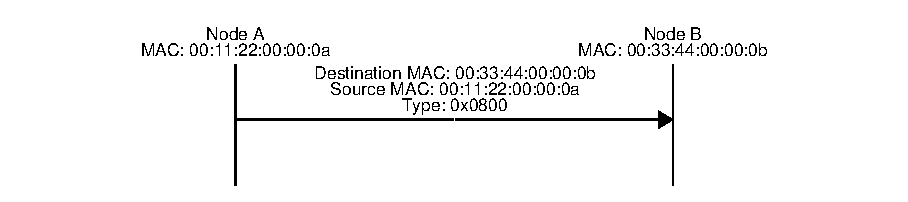
\includegraphics[width=\linewidth]{ethernet_message_unicast.eps}
\end{center}

Ethernet also supports \concept{broadcast} to all nodes in the LAN. In this case, the destination
MAC address must be \otherBase{ff:ff:ff:ff:ff:ff}.
% 
When a device receives a frame, it discards it unless the destination MAC field in the frame
is identical to its own MAC address, or \concept{broadcast}. 

A node will also discard a frame with an unsupported Payload Type (\concept{EtherType}) field. 
% 
If the payload type is supported, it is used to decide what part of the OS receives the message,
\eg, the \concept{IPv4} stack or the \concept{ARP} subsystem.

\begin{exercise} Continuing the example of the figure above, the network card of Node~B receives
a \concept{frame} that begins with the following bytes. Should it be accepted by B?
\begin{center}
\otherBase{00 11 22 00 \quad 00 0a ff ff \quad ff ff ff ff \quad 08 DD \ldots}
\end{center}
\end{exercise}

\begin{exercise}
The following scripts exemplify how to send and receive raw \concept{Ethernet} frames. 
The \concept{client} sends $5$ identical frames of \concept{EtherType} \otherBase{0x1234} and then exits.
The \concept{server} waits until it receives $5$ Ethernet frames of that type (checked in lines 12-13) and then exits.
% 
\begin{itemize}
\item Change the client's MAC address (see page \pageref{sec:layer2:practical}) and interface name with yours.
\item Make the server reject frames not addressed to it.
\item Extend these scripts to implement a simple application with \concept{LAN} capabilities.\\
  Suggested examples:
    \begin{itemize}
    \item A Layer-2 \concept{echo} service that distinguishes between petitions and responses.
    \item A Layer-2 \concept{peer-to-peer} chat that includes the origin's nickname in all messages.
    \item A Layer-2 calculator service that supports basic arithmetic operations\\
      (\inlineCode{+}, \inlineCode{-},\inlineCode{*}, integer division \inlineCode{//}, optionally division \inlineCode{/}).
    \end{itemize}
\item What is missing so that your application can connect to the rest of the \concept{Internet} beyond your \concept{LAN}?
\end{itemize}

\begin{remark}
You will need to run these scripts with privileges, \eg, with \inlineCode{sudo}.
% 
Alternatively, you can permanently add the \texttt{CAP\_NET\_RAW} capabilities
to your python binary with
\begin{center}
\inlineCode{sudo setcap cap_net_raw+ep ./venv/bin/python}.  
\end{center}
% 
After that, you can run \inlineCode{./venv/bin/python script.py} directly without \inlineCode{sudo}.\\[-0.5cm]
\end{remark}
\label{ex:layer2:echo}
\end{exercise}

\begin{center}
\showCode{snippets/ethernetclient.py}
\end{center}

\begin{center}
\showCode{snippets/ethernetserver.py}
\end{center}

% TODO: include something about the following aspects
% https://en.wikipedia.org/wiki/IEEE_802)
% wifi: https://en.wikipedia.org/wiki/IEEE_802.11#Layer_2_%E2%80%93_Datagrams
% ppp, ssh tunnels
% capture in monitor mode: https://wiki.wireshark.org/CaptureSetup/WLAN#linux
% usb protocol: https://en.wikipedia.org/wiki/USB_communications#Protocol_layer
\chapterimage{golden_gate.jpg}

\chapter{Layer 3: Internet(work) communication}\label{sec:layer3}

\begin{minipage}{0.4\linewidth}
\begin{center}
\begin{bytefield}{16}
\bitbox{16}{Layer 7: Application} \\
\bitbox{16}{Layer 4: Transport} \\
\bitbox{16}{\color{color1} Layer 3: Internet} \\
\bitbox{16}{Layer 2: Network (LAN)} \\
\bitbox{16}{Layer 1: Physical} \\
\end{bytefield}
\end{center}
\end{minipage}
\begin{minipage}{0.6\linewidth}
\begin{center}
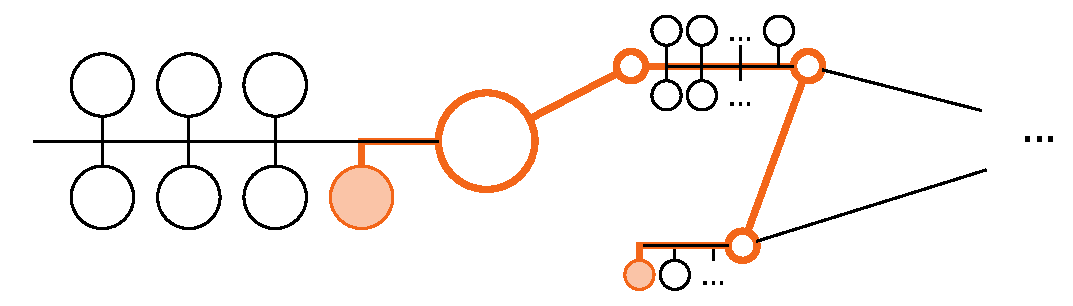
\includegraphics[width=\linewidth]{network_layer3.pdf}
\end{center}
\end{minipage}

\vspace{-0.75cm}

\subsection*{Capabilities}

The \conceptRef{IP}{Internet Protocol (IP)} allows exchanging \concept{datagrams} 
(Layer~3 \conceptRef{PDU}{PDUs}) between devices from different \conceptRef{LAN}{LANs}.
% 
Its addressing system identifies devices globally and makes it possible to 
\conceptRef{routing}{route} datagrams anywhere we need. 

Devices communicating via IP may belong to LANs
based on different technologies and with different types of \concept{MAC} address.
This has two implications:
\begin{itemize}
  \item A datagram that ``fits'' in the \concept{MTU} of the source LAN
    may be too large for the destination's (or any intermediate's) LAN MTU. 
    IP defines a \concept{fragmentation} system to split datagrams,
    which are reconstructed only at the final destination.\\[-0.25cm]
    
  \item When we send a datagram, we know the target device's \conceptRef{IP}{IP address},
  but not necessarily its \concept{MAC} address. Only if we are part of the destination
  LAN we will need that MAC. IP uses \concept{ARP} to translate known IP addresses
  to MAC addresses of the destination LAN's type.

\end{itemize}



\conceptRef{datagram}{Datagrams} may travel through networks not controlled 
by neither the source nor the destination, so datagrams may be lost, reordered and duplicated.
% 
Layer~3 does not provide mechanisms to deal with this; upper layers must implement
protection mechanisms when required 
(\eg, to implement \concept{TCP}'s \conceptRef{stream}{data streams}).


\vspace{-0.25cm}
\subsection*{Protocols}

Version~4 of \concept{IP} is \textit{the} protocol used in Layer~3, \ie,
it is common to virtually all communications in the Internet as we know it today.
% 
For many years, the Internet has been struggling to transition towards \concept{IPv6}, 
but the process is not complex and only \concept{IPv4} provides global coverage.

\concept{IPv4} delegates in the \concept{ARP} protocol the translation of known IP addresses 
into MAC addresses within each LAN. ARP does \textit{not} use IP datagrams.

The following protocols encapsulate their \conceptRef{PDU}{PDUs} in the payload of IP 
\conceptRef{datagram}{datagrams}:\\[-0.6cm]
\begin{itemize}
\item Transport Control Protocol (\concept{TCP}) 
\item User Datagram Protocol (\concept{UDP})
\item Internet Control Message Protocol (\concept{ICMP})
\end{itemize}


\subsection*{Addressing}

\concept{IPv4} addresses are $32$~bit long. They are most often presented to humans in
the \concept{quad decimal} format, \eg, \otherBase{142.250.201.67}. 

Most IP addresses are \conceptRef{public IP}{public} and unique across the Internet, 
\ie, the previous IP has the same meaning worldwide: it identifies a single connected device.

Many addresses are \conceptRef{private IP}{private}, have special meanings
and cannot be used for routing datagrams through the Internet, including:
\begin{itemize}
\item The \otherBase{127.*.*.*} and \otherBase{0.*.*.*} blocks cannot leave the local computer.
\item The \otherBase{172.*.*.*} and \otherBase{192.168.*.*} cannot leave the \concept{LAN}.
\item \otherBase{255.255.255.255} is reserved for the \concept{local IP broadcast} IP 
(used by \concept{DHCP}).
\end{itemize}

\begin{remark}
The same private address can be used by multiple devices if they belong to different LANs.
However, if that happens in the same LAN, communication may misbehave.
\end{remark}

\subsection*{Practical aspects}

The \inlineCode{ip address}, \inlineCode{ip route} and \inlineCode{ip neighbor} commands 
(among others) let you query several aspects of your IP configuration.

\begin{exercise}\ \\[-0.5cm]
\begin{itemize}
\item How many different \concept{IPv4} addresses are there (including reserved and private)? 
\item Are they sufficient now and in the future?
\item Is it problematic that an address like \otherBase{192.168.0.1} can be used by thousands
  of computers in the Internet right now?
\end{itemize}
\end{exercise}


\section{IP -- Internet Protocol}

\subsection*{Packet format}

\concept{IP} defines a \concept{packet} format with a \concept{header} 
that is \textit{at least} $20$~bytes long. Optional parts may be included,
as long as the total header size is a multiple of $32$~bits ($4$~bytes).
The payload can be empty, so the minimum datagram size is $20$~bytes.\\

\begin{center}
\small
\begin{bytefield}[bitheight=3em]{32}
\bitheader{0-31}\\
\begin{rightwordgroup}[curlyshrinkage=10pt]{Mandatory Header ($20$~bytes)}
  \bitbox{4}{IP\\Version} 
  & \bitbox{4}{IHL\\{\scriptsize(HLen/$4$)}} 
  & \bitbox{8}[bgcolor=lightgray]{Type of Service}
  & \bitbox{16}{Datagram Length\\{\scriptsize(Head + Payload, bytes)}} \\
  % 
  \bitbox{16}{Fragment ID} & \bitbox{1}{\otherBase{0}}
  & \bitbox{1}{\rotatebox{90}{\scriptsize DF flag}}
  & \bitbox{1}{\rotatebox{90}{\scriptsize MF flag}}
  & \bitbox{13}{Fragment Offset} \\
  % 
  \bitbox{8}{Time to Live\\(TTL)}
  & \bitbox{8}{Payload protocol}
  & \bitbox{16}[bgcolor=lightgray]{IP Header Checksum}\\
  % 
  \bitbox{32}{Source IP Address} \\
  \bitbox{32}{Destination IP Address}
\end{rightwordgroup} \\
%   
\begin{rightwordgroup}[curlyshrinkage=10pt]{Optional Header (32$\cdot x$ bits)}
\bitbox[tlr]{32}[bgcolor=lightgray]{Options\\{\scriptsize(variable length, optional)}} \\
\bitbox[lbr]{24}[bgcolor=lightgray]{} &
\bitbox{8}[bgcolor=lightgray]{Padding to\\$32$ bits}
\end{rightwordgroup} \\
% 
\begin{rightwordgroup}[curlyshrinkage=10pt]{Payload (8$\cdot y$ bits)}
\bitbox[tlr]{32}{Payload data} \\
\bitbox[lbr]{8}{} & \bitbox[t]{24}{} 
\end{rightwordgroup}
\end{bytefield}
\end{center}

\begin{exercise} \ \\[-0.5cm]
\begin{itemize}
\item How can the payload length be calculated from the header?
\item What is the maximum payload length?
\item What are the possible values of the flags in the IP header?
\item What's longer, an IP address or an Ethernet MAC address?
\item Is it possible to send exactly 17 bits of payload data in an IP datagram?
\item How can we know whether a datagram is encapsulating TCP or UDP data?
\item Why must the optional header part by a multiple of $32$~bits?
\end{itemize}
\end{exercise}


% \subsection{IP addresses, netmasks and CIDR format}\label{sec:layer3:cidr}
% also division
% 
% \subsection{Fragmentation}
% 
% \subsection{Routing}

\section{ARP -- Address Resolution Protocol}
\begin{remark}
The \concept{ARP} protocol does \textit{not} use IP headers.
\end{remark}

\section{ICMP -- Internet Control Message Protocol}


% - talk about the problem of having different networks, different technologoies (ARPA, XEROX
% - longest prefix matching for routing tables
% - first draft: 8-bit network addresses (a bit off!)

\chapterimage{tubes.jpg}

\chapter{Layer 4: Transport}\label{sec:layer4}

\begin{minipage}{0.4\linewidth}
\begin{center}
\begin{bytefield}{16}
\bitbox{16}{Layer 7: Application} \\
\bitbox{16}{\color{color1} Layer 4: Transport} \\
\bitbox{16}{Layer 3: Internet} \\
\bitbox{16}{Layer 2: Network (LAN)} \\
\bitbox{16}{Layer 1: Physical} \\
\end{bytefield}
\end{center}
\end{minipage}
\begin{minipage}{0.6\linewidth}
\begin{center}
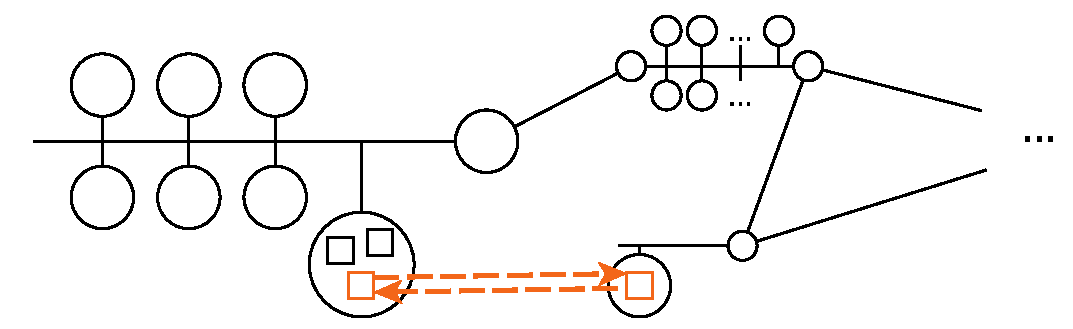
\includegraphics[width=\linewidth]{network_layer4.pdf}
\end{center}
\end{minipage}


% la ventana controla el flujo porque, si envio y recivo rápido, - envío el siguiente paquete antes, y sé que puedo porque la otra parte confirma al mismo ritmo.

\chapter{Layer 7: Application communication}

% - client vs server (in TCP/IP, symmetry)?
% - server-client model
% - global structure, ownership and organization, 

% TODO: add  somewhere
%  - history timeline
% - first draft: 8-bit network addresses (a bit off!)
%  - a section where stuff like NAT, firewall, IDS, etc. can be introduced?

% TODO: timeline points
% \begin{remark}
% Many interesting historical reviews of the creation of the Internet are available online,
% \eg, \href{https://www.youtube.com/watch?v=oIezCGjxV3A}{\underline{this video}}.
% Some events of particular importance are:
% \begin{itemize}
% \item[\textbf{1962}: ] Packet Switching
% \item[\textbf{1969}: ] ARPANET
% \item[\textbf{1974}: ] TCP/IP
% \item[\textbf{1986}: ] IETF
% Pat Thaler: chairwoman 802.3 10BASE-T (twisted pair) (https://www.youtube.com/watch?v=f8PP5IHsL8Y
% \item[\textbf{1991}: ] WWW
% \item[\textbf{1993}: ] CIDR addressing
% \item[\textbf{1998}: ] Google
% % - How about 2016 IANA?
% \end{itemize}
% \end{remark}

% TODO: auto-populate a file with problem-friendly exercises

% TODO: populate this chapter with the code-related exercises
% \chapter{Labs}

\begin{enumerate}

\item Platform setup, bit-byte with python, basis for submask calculator (extend snippets/bitwisemanipulation.py?)


\end{enumerate}


% \begin{itemize}
% \item 
% \end{itemize}
% \begin{enumerate}
% \item 
% \end{enumerate}


% %----------------------------------------------------------------------------------------
%	BIBLIOGRAPHY
%----------------------------------------------------------------------------------------

\chapter{Bibliography}

\todo[inline]{Makefile does not compile this because there is nothing to do}

% \addcontentsline{toc}{chapter}{\textcolor{color1}{Bibliography}}
\section*{Books}
% \addcontentsline{toc}{section}{Books}
\printbibliography[heading=bibempty,type=book]
\section*{Articles}
% \addcontentsline{toc}{section}{Articles}
\printbibliography[heading=bibempty,type=article]

% Indices, tables of contents, etc.



%----------------------------------------------------------------------------------------
%	INDEX
%----------------------------------------------------------------------------------------

% \indexsetup{level=\section*,toclevel=section,noclearpage}

\chapterimage{word_list.jpg}
\chapter*{Index of Concepts}

\indexprologue{}
% \indexprologue{\noindent (You can clink on the page numbers to go to the sections where each concept is used)}
\printindex
% \printindex[names]
% \printindex[objects]

% % % % \cleardoublepage
% % % \phantomsection
% % % % \setlength{\columnsep}{0.75cm}
% % % \section*{Index of Concepts}
% % % % \addcontentsline{toc}{chapter}{\textcolor{color1}{Index}}
% % % \ \\
% % % \ \\
% % % xxxx
% % % \ \\
% % % \ \\
% % % \printindex
% Vamos

%----------------------------------------------------------------------------------------


% PEnding:


\begin{comment}
% Plan plan plan:
% 
% unas cuantas sesiones hablando de los problemas
% 
% al cabo de un mes o así deadline de propuesta de diseño:
%     - un documento respondiendo a las principales preguntas (el documento las plantea)
%     - después del deadline, se asigna y se usa para comparar (notas entre ellos para la nota de clase)

\end{comment}

\end{document}
